% !TeX root = ../../Book1.tex
% 纲要标题：## 第8章　曲面的基本形式、相容条件与局部实现
% 纲要位置：几何学计划纲要.md，第 398 行。
% 正文状态：初稿；尚未正式审核。

% 纲要内容开始
% 
% > 本章目标与证明范围：完整建立从浸入到两基本形式、再由相容数据恢复浸入的双向理论。第一基本形式不再独立为浅章；Gauss–Codazzi 的必要性和局部存在性分别展开。
% 
% 纲要内容结束

\chapter{曲面的基本形式、相容条件与局部实现}
\label{g1:ch:08}
\BookChapterNumber{g1:ch:08}

\begin{chapterabstract}
	一张曲面同时携带沿面测量的度量与在空间中弯曲的法向数据。本章从正则参数、切平面与坐标变换建立两种基本形式，推导长度、面积、微分算子和主曲率的计算方法，再以混合偏导相容性联系内在曲率与外在弯曲。反向构造从光滑正定度量及对称第二基本形式出发：相容方程使标架系统可积分，闭的候选微分再恢复位置，从而得到曲面基本定理的局部存在与唯一性。最后用球面、圆柱、旋转曲面及一阶形变说明数据、法向、局部实现和整体刚性各自的作用。
\end{chapterabstract}

\begin{learninggoals}
	\begin{itemize}
		\item 从参数映射检查浸入条件，求两种基本形式，并在换参数或换法向后正确转换数据。
		\item 利用第一基本形式计算长度、面积、梯度、散度及本书符号约定下的 Laplace 算子，辨别局部等距与环境刚性运动。
		\item 求形算子、主曲率、平均曲率与法曲率，判断脐点及渐近方向，并说明点态方向与局部积分曲线的区别。
		\item 从切向投影推导结构方程，证明曲率由度量决定，并分清两组相容条件各自排除的障碍。
		\item 通过矩形上的标架积分和位置积分重建曲面，核验秩、法向、两种形式及初值唯一性。
		\item 用明确算例区分局部存在、整体单值、整体单射与一阶形变。
	\end{itemize}
\end{learninggoals}

在平面纸片上画一个小三角形，再把纸片卷成圆柱的一部分，它的三条边沿纸测量时仍可保持原来的长度，但空间中的三个顶点及其切平面已经改变。这个例子提出两个问题：哪些数据描述纸片内部的测量，哪些数据描述它在空间中的摆放？反过来，如果只给出这两类数据，是否总能找到一个曲面把它们实现出来？

\ProseParagraphBreak

第一类数据来自两个参数切向量的内积，即第一基本形式；第二类来自法向量随位置的改变，即第二基本形式。后者不是任意的三个函数。一个位置函数 \(X(u,v)\) 同时沿两个方向变化，混合偏导必须相等，因此长度和弯曲数据要满足相容方程。曲线的重建只需沿一条参数线解常微分方程；曲面的重建则还要证明，先横走后竖走与相反次序不会给出冲突的标架。

\ProseParagraphBreak

本章将这一步直接落实为积分证明：先归一化待求标架，再建立矩形上的双变量系统，最后对两个候选切向量积分得到位置。正定性用于保证得到的是浸入；相容性用于消除混合偏导的冲突；指定初值用于说明唯一性。绕环路后的标架与位移另作检查，因为每个小邻域能够实现，并不保证带孔区域上存在单值实现。

\ProseParagraphBreak

所需基础是多元微积分中的链式法则、偏导交换、Taylor 展开、积分换元与分部积分，以及内积和矩阵运算。局部逆映射的所需版本、二维自伴算子的主方向、局部积分曲线和双变量系统的存在性均在本章证明。第七章的长度公式和线性方程引理将在使用处回顾。参数曲面、两种基本形式和曲率的延伸阅读可查 Pressley 第二版的明确位置\cite[第4.1--4.5, 6.1--6.2, 7.1--7.3, 8.1--8.2, 10.1--10.2节]{Pressley2010}。

% !TeX root = ../../Book1.tex
% 纲要标题：### 8.1 正则曲面和度量数据
% 纲要位置：几何学计划纲要.md，第 402 行。
% 正文状态：初稿；尚未正式审核。

% 纲要内容开始
% 
% * 浸入参数、图像模型和切平面
% * 第一基本形式的坐标变换
% * 长度、面积和局部等距
% * 梯度、散度与曲面上的微分算子
% 
% 纲要内容结束

\section{正则曲面和度量数据}
\label{g1:sec:0801}

把一张纸弯成圆柱的一部分，纸上两条相交曲线的夹角和沿纸测量的长度可以保持不变，纸在空间中的法方向却已经改变。要把这两种现象分开，首先应弄清参数怎样记录曲面，以及哪些计算只需两个切向量的内积。本章均在光滑即 \(C^\infty\) 的范围内讨论；这使后面交换偏导与求解标架系统时无需反复改变正则性条件，并不表示每一条单独的公式都需要无限次可微。

\subsection{浸入参数、图像模型和切平面}
\label{g1:subsec:0801:01}

曲线的正则性要求速度不为零，曲面的对应要求是两个参数方向不能塌缩成一条直线。以下记 \(u^1=u,u^2=v\)，\(\partial_i=\partial/\partial u^i\)，\(X_i=\partial_iX\)。

\begin{definition}[正则参数曲面]\label{g1:def:surface-immersion}
	设 \(U\subseteq\mathbb R^2\) 开。光滑映射 \(X:U\rightarrow\mathbb R^3\) 若处处满足 \(\operatorname{rank}\mathrm{d}X=2\)，称为一个\term[zhengzecanshuqumian]{正则参数曲面}[regular parametrized surface]，也称参数域到 \(\mathbb R^3\) 的\term[jinru]{浸入}[immersion]。等价地，\(X_1,X_2\) 线性无关，或 \(X_1\times X_2\ne0\)。在参数点 \(q\in U\) 处的\term[qiepingmian]{切平面}[tangent plane]作为向量空间定义为
	\[
		\mathrm{T}_qX\coloneqq \mathrm{d}X_q(\mathbb R^2)=\operatorname{span}\{X_1(q),X_2(q)\}.
	\]
	经过曲面点的仿射切平面是 \(X(q)+\mathrm{T}_qX\)。若两个参数点具有同一空间像，记号 \(\mathrm{T}_qX\) 仍记录所选参数点，而不擅自把两个分支的切平面等同。
\end{definition}

最直接的模型是图像 \(X(u,v)=(u,v,f(u,v))\)：前两个分量已经保证两个偏导线性无关。反过来，每个浸入在足够小的参数邻域内都能换成这样的模型。为免把“选适当坐标”隐藏为一句话，先说明这里需要的逆映射事实。

\begin{lemma}[局部逆映射的一个版本]\label{g1:lem:surface-local-inverse}
	设 \(f:V\rightarrow\mathbb R^m\) 光滑，\(V\subseteq\mathbb R^m\) 开，且 \(\mathrm{D}f(a)\) 可逆。则 \(a\) 有开邻域 \(V_0\)，使 \(f|_{V_0}\) 是到某个开集的光滑双射，逆映射也光滑。
\end{lemma}

\begin{proof}
	平移并左乘 \(\mathrm{D}f(a)^{-1}\)，可设 \(a=0,f(0)=0,\mathrm{D}f(0)=I\)。取闭球 \(\overline B_r\subset V\)，使其中 \(\|\mathrm{D}f-I\|\le q<1\)。沿线段积分导数得到
	\[
		\|f(x)-f(z)-(x-z)\|\le q\|x-z\|,\qquad
		\|f(x)-f(z)\|\ge(1-q)\|x-z\|.
	\]
	对 \(\|y\|<(1-q)r\)，映射 \(\Phi_y(x)=y+x-f(x)\) 将闭球映入自身，且距离至多缩短为原来的 \(q\) 倍。从球内任一点迭代，相邻两项的距离至多为 \(q^j\) 倍初始距离，故迭代列为 Cauchy 列；闭球完备，极限 \(x\) 满足 \(f(x)=y\)。同一缩短估计证明解唯一。令 \(V_0=B_r\cap f^{-1}(B_{(1-q)r})\)，便得所需双射；上面的第二个不等式使逆映射连续且局部 Lipschitz。

	写 \(x=f^{-1}(y)\) 及 \(x+h=f^{-1}(y+k)\)。由 \(k=\mathrm{D}f(x)h+o(\|h\|)\) 和 \(\|h\|\le(1-q)^{-1}\|k\|\)，有
	\[
		h=\mathrm{D}f(x)^{-1}k+o(\|k\|).
	\]
	因此逆映射可微，导数为 \(\mathrm{D}f(f^{-1}(y))^{-1}\)，且连续。对这个表达式反复求导，依次得到全部高阶连续导数。恢复最初的平移和可逆线性变换即得结论。
\end{proof}

\begin{proposition}[浸入的局部图像]\label{g1:prop:surface-local-graph}
	设 \(X:U\rightarrow\mathbb R^3\) 为光滑浸入，\(q\in U\)。选择空间中适当的两个坐标后，\(q\) 有邻域 \(U_0\)，使 \(X(U_0)\) 是这两个坐标上的光滑函数图像；\(X|_{U_0}\) 是到其像的同胚。其切平面恰为所有通过 \(q\) 的光滑参数曲线在空间中的速度所组成的集合。特别地，可先用刚性运动把该点移到原点、切平面移成水平面，再得到满足 \(f(0)=0,\mathrm{d}f(0)=0\) 的图像。
\end{proposition}

\begin{proof}
	矩阵 \(\mathrm{d}X_q\) 的秩为二，故某个二阶子式不为零。设对应前两个空间坐标，令 \(\pi(x,y,z)=(x,y)\)。由前一引理，\(\pi\circ X\) 在较小邻域内有光滑逆 \(\psi\)。于是
	\[
		X\circ\psi(x,y)=(x,y,f(x,y)).
	\]
	图像的逆坐标是连续的投影 \(\pi\)，所以原参数映射在该邻域内也是同胚。参数曲线 \(c(t)\) 满足 \(c(0)=q\) 时，\((X\circ c)'(0)=\mathrm{d}X_q(c'(0))\) 属于上述张成空间；反之，每个 \(\mathrm{d}X_q(w)\) 都由短直线 \(c(t)=q+tw\) 实现。若先将切平面移为水平面，投影 \(\pi\) 限制在该切平面上就是线性同构，所以上述逆映射论证仍适用；图像的水平切平面又使两个一阶偏导都为零。
\end{proof}

若子集 \(S\subseteq\mathbb R^3\) 在每一点附近都恰好是一个这样的图像，称为\term[zhengzequmian]{正则曲面}[regular surface]，此时也称嵌入曲面。它的图像参数之间的过渡映射光滑，因为可写为一张图像的投影与另一张参数映射的复合。浸入只保证每个参数分支局部如此，不保证整个像是嵌入曲面。例如
\[
	X(u,v)=(\sin u,\sin2u,v),\qquad (u,v)\in\mathbb R^2
\]
处处为浸入：\((\cos u,2\cos2u)\) 不会同时为零。但 \(u=0\) 与 \(u=\pi\) 的分支在同一竖直线上相交，两个切平面不同。本章的局部计算始终在选定分支上进行。

\subsection{第一基本形式的坐标变换}
\label{g1:subsec:0801:02}

参数方向 \(a=(a^1,a^2)\) 本身的欧氏长度通常不是曲面上相应速度的长度。实际速度是 \(a^1X_1+a^2X_2\)，其平方范数把所需数据集中为一个二次型。

\begin{definition}[第一基本形式]\label{g1:def:first-fundamental-form}
	设 \(X:U\rightarrow\mathbb R^3\) 为光滑浸入。定义
	\[
		g_{ij}=\langle X_i,X_j\rangle,\qquad
		E=g_{11},\quad F=g_{12}=g_{21},\quad G=g_{22},\quad D=EG-F^2.
	\]
	参数方向上的内积 \(g(a,b)=\sum_{i,j=1}^2g_{ij}a^ib^j\) 称为曲面的\term[diyijibenxingshi]{第一基本形式}[first fundamental form]，记
	\[
		I=E\,\mathrm{d}u^2+2F\,\mathrm{d}u\,\mathrm{d}v+G\,\mathrm{d}v^2.
	\]
	这里 \(\mathrm{d}u^2\) 表示 \(\mathrm{d}u\otimes \mathrm{d}u\) 在同一向量上求值所得的平方，混合项同理；它不是对参数函数取二阶导数。第一基本形式在每点正定，故 \(E>0,D>0\)。
	\symidx{\(g_{ij}\)：第一基本形式的系数}
	\symidx{\(I\)：第一基本形式}
\end{definition}

\begin{proposition}[度量的换元公式]\label{g1:prop:surface-metric-change}
	设 \(X:U\rightarrow\mathbb R^3\) 为光滑浸入，\(\phi:\widetilde U\rightarrow U\) 为光滑微分同胚，即光滑且有光滑逆的双射。置 \(\widetilde X=X\circ\phi\)，以 \(J=(\partial u^i/\partial\widetilde u^a)\) 记换元导数矩阵。则
	\begin{equation}\label{g1:eq:surface-metric-change}
		\widetilde g=J^{\mathsf T}(g\circ\phi)J,\qquad
		\det\widetilde g=(\det J)^2(D\circ\phi).
	\end{equation}
	特别地，\(g\) 的正定性以及相应切向量之间的长度和夹角不依赖坐标。
\end{proposition}

\begin{proof}
	链式法则给出 \(\widetilde X_a=\sum_iX_i\,\partial_a\phi^i\)。两边取内积即为第一式，再取行列式即为第二式。若同一参数方向在两坐标中的分量满足 \(a=J\widetilde a\)，则 \(\widetilde a^{\mathsf T}\widetilde g\widetilde b=a^{\mathsf T}gb\)，这也直接说明所有内积计算保持一致。
\end{proof}

因此，度量不是某张矩阵本身，而是按这一规律相互转换的一族内积。即使暂时没有空间中的曲面，参数域上的任意光滑正定对称矩阵场也定义一个\term[limanduliang]{黎曼度量}[Riemannian metric]；本章重建问题正是询问这样的 \(g\) 与另一个对称数据 \(h\) 能否同时来自浸入。此名称所指的内在度量与环境空间中的欧氏距离应区分。\footnote{Riemann，黎曼，德文全名 Georg Friedrich Bernhard Riemann（1826--1866），德国数学家，在复分析、几何及分析学中作出基础性贡献。}

\begin{example}[坐标网格可以不正交]\label{g1:exm:oblique-plane-metric}
	平面参数 \(X(u,v)=(u+v,v,0)\) 给出 \(E=1,F=1,G=2\)，所以 \(I=\mathrm{d}u^2+2\,\mathrm{d}u\,\mathrm{d}v+2\,\mathrm{d}v^2\)。两个参数轴在空间中的夹角余弦为 \(1/\sqrt2\)，而不是零。另一方面，参数 \(X(r,\theta)=(r\cos\theta,r\sin\theta,0)\) 在 \(r>0\) 时给出 \(I=\mathrm{d}r^2+r^2\mathrm{d}\theta^2\)。系数变化可能仅来自坐标；这两张矩阵都描述平面的欧氏度量。
\end{example}

\subsection{长度、面积和局部等距}
\label{g1:subsec:0801:03}

度量的用途先从测量开始。若 \(c:[a,b]\rightarrow U\) 分段 \(C^1\)，空间曲线的速度为 \(\mathrm{d}X(c')\)，由\cref{g1:prop:arc-length-param}中的长度积分公式，
\begin{equation}\label{g1:eq:surface-length}
	L_g(c)=\int_a^b\sqrt{\sum_{i,j}g_{ij}(c(t))\dot c^i(t)\dot c^j(t)}\,\mathrm{d}t.
\end{equation}
两非零方向 \(a,b\) 的夹角余弦为 \(g(a,b)/\sqrt{g(a,a)g(b,b)}\)。这里距离沿曲面测量；将两点在空间中直线相连所得到的弦长一般不等于沿面的最短路程。

\begin{definition}[面积密度]\label{g1:def:surface-area-density}
	对光滑浸入 \(X:U\rightarrow\mathbb R^3\)，其\term[mianjimidu]{面积密度}[area density]及参数区域 \(A\subset U\) 的面积定义为
	\[
		\mathrm{d}A_g=\sqrt D\,\mathrm{d}u\,\mathrm{d}v,\qquad
		\operatorname{Area}_X(A)=\int_A\sqrt D\,\mathrm{d}u\,\mathrm{d}v,
	\]
	其中 \(A\) 可取紧包含于 \(U\) 的分片光滑有界区域。若不同参数部分覆盖同一空间部分，此积分计入覆盖次数。
\end{definition}

这个因子的几何来源是微分 \(\mathrm{d}X\) 把参数单位小正方形送成由 \(X_1,X_2\) 张成的平行四边形，而
\[
	\|X_1\times X_2\|^2=\|X_1\|^2\|X_2\|^2-\langle X_1,X_2\rangle^2=D.
\]
面积定义使用微分给出的局部伸缩；并不声称随意选取的空间多面体逼近，其面积都自动收敛到这个值。由\eqref{g1:eq:surface-metric-change}，\(\sqrt{\det\widetilde g}=\sqrt{D\circ\phi}\,|\det J|\)，结合多元积分换元公式便知面积不依赖参数。换元公式在这里的具体用途是：可微双射的导数行列式绝对值恰补偿参数区域面积的改变。

\begin{definition}[局部等距]\label{g1:def:surface-local-isometry}
	设 \(U,V\subseteq\mathbb R^2\) 带光滑正定度量 \(g,\widetilde g\)。光滑映射 \(\phi:U\rightarrow V\) 若在每点附近为微分同胚，且
	\[
		g_q(a,b)=\widetilde g_{\phi(q)}(\mathrm{d}\phi_q(a),\mathrm{d}\phi_q(b))
	\]
	对所有 \(q,a,b\) 成立，称为\term[jubudengju]{局部等距}[local isometry]。对嵌入曲面的映射，在局部参数中采用同一定义。若映射在整体上是微分同胚并满足此式，则称为两度量曲面的等距。
\end{definition}

\begin{proposition}[长度刻画局部等距]\label{g1:prop:local-isometry-length}
	设 \(\phi:(U,g)\rightarrow(V,\widetilde g)\) 为光滑局部微分同胚。则 \(\phi\) 是局部等距，当且仅当每条分段 \(C^1\) 参数曲线 \(c\) 都满足 \(L_{\widetilde g}(\phi\circ c)=L_g(c)\)。局部等距还保持夹角及在单射邻域内计算的面积。
\end{proposition}

\begin{proof}
	保持内积直接给出速度模相同，积分即得长度相同；夹角公式和度量行列式的换元式给出另两项。反过来，固定 \(q\) 与方向 \(a\)，取短线段 \(c(t)=q+ta\)，\(0\le t\le\varepsilon\)。将长度相等除以 \(\varepsilon\)，令 \(\varepsilon\to0^+\)，连续性给出 \(g_q(a,a)=\widetilde g_{\phi(q)}(\mathrm{d}\phi_q(a),\mathrm{d}\phi_q(a))\)。利用
	\[
		2g(a,b)=g(a+b,a+b)-g(a,a)-g(b,b)
	\]
	恢复全部内积，故得局部等距。
\end{proof}

这个定义比较的是切向量及沿面测量，不要求 \(\phi\) 是环境空间某个刚性运动的限制。\subsecref{g1:subsec:0805:02}会用圆柱把这一区别算出来。局部等距也不保证整体单射，因而不能将局部保持长度直接理解为全局最短距离和拓扑都不改变。

\subsection{梯度、散度与曲面上的微分算子}
\label{g1:subsec:0801:04}

已知一个温度函数 \(f\)，沿方向 \(a\) 的变化率 \(\mathrm{d}f(a)=\sum_i(\partial_i f)a^i\) 不需要度量；但问“沿哪个单位方向增长最快”，就必须知道什么叫单位长度。反过来，描述切向流的局部流出量时，还必须使用正确的面积密度。这两点分别导出梯度与散度。

\begin{definition}[梯度]\label{g1:def:surface-gradient}
	在带光滑正定度量 \(g\) 的平面开集 \(U\) 上，光滑函数 \(f\) 的\term[tidu]{梯度}[gradient]是唯一满足 \(g(\operatorname{grad}_g f,a)=\mathrm{d}f(a)\) 的向量场。若 \(g^{-1}=(g^{ij})\)，则
	\begin{equation}\label{g1:eq:surface-gradient}
		\operatorname{grad}_g f=\sum_{i,j}g^{ij}(\partial_j f)\partial_i.
	\end{equation}
	在浸入曲面上，右端的 \(\partial_i\) 经 \(\mathrm{d}X\) 对应到 \(X_i\)。
\end{definition}

求解线性方程 \(g_{ij}(\operatorname{grad}f)^j=\partial_i f\) 就得到公式。它说明直接把两个偏导数当作梯度分量，只有在度量矩阵为单位阵的坐标中才正确。若梯度非零，Cauchy--Schwarz 不等式给出 \(\mathrm{d}f(a)\le\|\operatorname{grad}f\|_g\)（\(\|a\|_g=1\)），等号在梯度方向达到；若 \(f\) 是环境函数 \(\widehat f\) 的限制，曲面梯度恰为欧氏梯度 \(\nabla\widehat f\) 的切向正交投影，因为两者与任何切向量的内积都等于该方向导数。

\begin{definition}[散度与 Laplace 算子]\label{g1:def:surface-divergence-laplacian}
	设 \(g\) 为 \(U\subseteq\mathbb R^2\) 上的光滑正定度量，\(W=\sum_iW^i\partial_i\) 为光滑向量场。定义其\term[sandu]{散度}[divergence]为
	\begin{equation}\label{g1:eq:surface-divergence}
		\operatorname{div}_gW=\frac1{\sqrt D}\sum_i\partial_i(\sqrt D\,W^i).
	\end{equation}
	函数上的\term[LaplaceBeltramisuanzi]{Laplace--Beltrami 算子}[Laplace--Beltrami operator]采用本书的非负号约定：
	\begin{equation}\label{g1:eq:surface-laplacian}
		\Delta_g f=-\operatorname{div}_g\operatorname{grad}_g f
		=-\frac1{\sqrt D}\sum_{i,j}\partial_i\bigl(\sqrt D\,g^{ij}\partial_jf\bigr).
	\end{equation}
	\symidx{\(\Delta_g\)：非负号约定的 Laplace--Beltrami 算子}
\end{definition}

上述名称分别纪念 Laplace 和 Beltrami。\footnote{Laplace，拉普拉斯，法文全名 Pierre-Simon Laplace（1749--1827），法国数学家和天文学家，研究概率、势函数与天体力学。Beltrami，贝尔特拉米，意大利文名 Eugenio Beltrami（1835--1900），意大利数学家，研究微分几何、非欧几何模型及微分算子。}为看清散度为何需要 \(\sqrt D\)，取紧支于 \(U\) 内的光滑函数 \(\eta\)，记作 \(\eta\in C_c^\infty(U)\)。通常的分部积分没有边界项，因此
\begin{equation}\label{g1:eq:surface-divergence-weak}
	\int_U\eta\,\operatorname{div}_gW\,\mathrm{d}A_g
	=-\int_U \mathrm{d}\eta(W)\,\mathrm{d}A_g.
\end{equation}
右边只涉及方向导数和已证明与坐标无关的面积，因而不依赖坐标。这一等式还唯一确定连续函数 \(\operatorname{div}_gW\)：若两个候选的差在一点为正，则在一个小圆盘上仍为正，在该圆盘取非负且不恒零的光滑函数作 \(\eta\)，便与积分为零矛盾。这样的函数可以显式取为圆盘内的 \(\exp(-1/(r^2-\|x-a\|^2))\)，在圆盘外取零；负值情形同理。于是散度公式确实定义了一个内在的标量，而不是坐标的偶然组合。

\begin{proposition}[非负号约定与局部等距]\label{g1:prop:surface-laplacian-energy}
	设 \(g\) 为平面开集 \(U\) 上的光滑正定度量，\(f,\eta\in C_c^\infty(U)\)。则
	\[
		\int_U\eta\Delta_g f\,\mathrm{d}A_g
		=\int_U g(\operatorname{grad}_g\eta,\operatorname{grad}_gf)\,\mathrm{d}A_g,
		\qquad
		\int_Uf\Delta_g f\,\mathrm{d}A_g\ge0.
	\]
	若 \(\phi:(U,g)\rightarrow(V,\widetilde g)\) 为光滑局部等距，则每个光滑函数 \(f\) 满足 \(\Delta_g(f\circ\phi)=(\Delta_{\widetilde g}f)\circ\phi\)。
\end{proposition}

\begin{proof}
	第一式在\eqref{g1:eq:surface-divergence-weak}中令 \(W=\operatorname{grad}f\) 并使用梯度的定义；令 \(\eta=f\) 得到第二式。对局部等距，定义直接给出 \(\mathrm{d}\phi(\operatorname{grad}_g(f\circ\phi))=(\operatorname{grad}_{\widetilde g}f)\circ\phi\)。在 \(\phi\) 单射的小邻域中，用面积换元和\eqref{g1:eq:surface-divergence-weak}可知相对应向量场的散度也对应。将两项结合即得算子等式；等式是逐点的，所以这些邻域足够覆盖整个定义域。
\end{proof}

“非负”说的是积分二次型，不是说 \(\Delta_g f\) 对每个 \(f\) 都逐点非负。在平面的极坐标中，\(g=\operatorname{diag}(1,r^2)\)、\(\sqrt D=r\)，故
\[
	\operatorname{grad}f=f_r\partial_r+\frac{f_\theta}{r^2}\partial_\theta,\quad
	\operatorname{div}W=\frac1r\partial_r(rW^r)+\partial_\theta W^\theta,\quad
	\Delta f=-f_{rr}-\frac1rf_r-\frac1{r^2}f_{\theta\theta}.
\]
例如 \(f=r^2\) 时 \(\Delta f=-4\)。这些式子只在 \(r>0\) 的极坐标区域使用；原点处公式的分母反映坐标失效，不能据此断言平面的几何有奇点。

% !TeX root = ../../Book1.tex
% 纲要标题：### 8.2 法向几何与第二基本形式
% 纲要位置：几何学计划纲要.md，第 409 行。
% 正文状态：初稿；尚未正式审核。

% 纲要内容开始
% 
% * Gauss 映射和形算子
% * 主曲率、法曲率与 Euler 公式
% * 平均曲率、Gauss 曲率及脐点
% * 曲率线、渐近线及其退化
% 
% 纲要内容结束

\section{法向几何与第二基本形式}
\label{g1:sec:0802}

一张纸卷成圆柱后，小范围内的长度和角度没有改变，切平面却随着位置转动。第一基本形式记录前一种信息；要描述后一种变化，就应比较邻近点的法向量。曲线只有一个切方向，曲面在一点有整整一圈方向，因此需要一个线性算子同时记录沿各方向前进时法向量怎样变化。以下所有曲面参数均为光滑浸入 \(X:U\to\mathbb R^3\)，其中 \(U\subset\mathbb R^2\) 为开集；讨论在参数邻域中进行，自交处的不同分支分别处理。

\subsection{Gauss 映射和形算子}
\label{g1:subsec:0802:01}

令 \(X_i=\partial X/\partial u^i\)。上一节的正则性保证 \(X_1\times X_2\ne0\)，因而在每张参数片上可以选择光滑单位法向
\[
	n=\frac{X_1\times X_2}{\sqrt D},\qquad
	D=EG-F^2,\quad E=\langle X_1,X_1\rangle,\quad F=\langle X_1,X_2\rangle,\quad G=\langle X_2,X_2\rangle.
\]
也可以选相反的 \(n\)。以下先固定这一选择；曲面若不能作整体的法向选择，这些构造仍可在每张小参数片上使用。

\begin{definition}[Gauss 映射与形算子]\label{g1:def:shape-operator}
	设 \(X:U\to\mathbb R^3\) 为光滑浸入，\(n:U\to S^2\) 为一个光滑单位法向场。把每一点送到其单位法向的映射 \(n\) 称为\term[Gaussyingshe]{Gauss 映射}[Gauss map]。\footnote{Gauss（高斯，Carl Friedrich Gauss，1777--1855）是德国数学家，在数论、微分几何与测地学等领域作出重要贡献。}对每个参数点 \(q\in U\)，令 \(p=X(q)\)，并在这一参数分支上定义\term[xingsuanzi]{形算子}[shape operator]
	\[
		S_q:\mathrm{T}_qX\longrightarrow \mathrm{T}_qX,\qquad
		S_q\!\left(\sum_i a^iX_i\right)=-\sum_i a^i n_i.
	\]
	它也记为 \(S=-\mathrm dn\)，其中用 \(\mathrm dX\) 把参数切向量与曲面切向量对应起来。
	\symidx{\(S\)：曲面的形算子 \(S=-\mathrm dn\)}
\end{definition}

这个定义中有两个需要核对的地方。首先，\(X_1,X_2\) 线性无关，所以系数 \(a^i\) 唯一；其次，对 \(\langle n,n\rangle=1\) 求导得到 \(\langle n_i,n\rangle=0\)，故 \(n_i\) 确实落在 \(\mathrm{T}_qX=n^\perp\) 中。Gauss 映射的微分本来取值于 \(\mathrm{T}_{n(q)}S^2\)，这里使用了这两个切平面作为 \(\mathbb R^3\) 线性子空间恰好都是 \(n^\perp\) 的事实。

\ProseParagraphBreak

负号使“曲线的法向加速度”稍后直接等于形算子的二次型。它也决定了球面的符号：半径 \(R\) 的球面若取外向法向 \(n(q)=p/R\)，则 \(\mathrm dn(v)=v/R\)，所以 \(S=-I/R\)。不要把别处采用 \(S=\mathrm dn\) 的主曲率公式直接移入这里。

\begin{definition}[第二基本形式]\label{g1:def:second-fundamental-form}
	在带选定单位法向的光滑浸入曲面上，对每个参数点 \(q\) 定义
	\[
		\mathrm{II}_q(v,w)\coloneqq\langle S_qv,w\rangle,\qquad v,w\in \mathrm{T}_qX.
	\]
	这个双线性型称为\term[dierjibenxingshi]{第二基本形式}[second fundamental form]。它的对称性由下面的计算给出。在坐标中记 \(h_{ij}=\mathrm{II}(X_i,X_j)\)，于是
	\[
		\mathrm{II}=h_{11}(\mathrm du^1)^2+2h_{12}\,\mathrm du^1\mathrm du^2+h_{22}(\mathrm du^2)^2.
	\]
	\symidx{\(\mathrm{II}\)：第二基本形式}
	\symidx{\(h_{ij}\)：第二基本形式的坐标系数}
\end{definition}

\begin{proposition}[形算子的自伴性与坐标表示]\label{g1:prop:shape-self-adjoint}
	设 \(X:U\to\mathbb R^3\) 为光滑浸入，并选定光滑单位法向 \(n\)。则
	\begin{equation}\label{g1:eq:second-form-coefficients}
		h_{ij}=-\langle n_i,X_j\rangle=\langle X_{ij},n\rangle.
	\end{equation}
	第二基本形式对称，形算子关于第一基本形式自伴，即 \(\langle Sv,w\rangle=\langle v,Sw\rangle\)。以列向量表示系数时，形算子在基 \(X_1,X_2\) 下的矩阵为
	\begin{equation}\label{g1:eq:shape-matrix}
		[S]=g^{-1}h,\qquad g=(g_{ij}),\quad h=(h_{ij}).
	\end{equation}
	若作光滑坐标变换 \(u=u(v)\)，令 \(A=(\partial u^i/\partial v^a)\)，并保留同一个几何法向场，则 \(\widetilde h=A^{\mathsf T}hA\)。因此 \(\mathrm{II}\) 不依赖参数的选择。
\end{proposition}
\begin{proof}
	对 \(\langle n,X_j\rangle=0\) 关于 \(u^i\) 求导，得到 \(\langle n_i,X_j\rangle+\langle n,X_{ij}\rangle=0\)。混合偏导相等给出 \(h_{ij}=h_{ji}\)，再由双线性性得到自伴性。若 \(S(X_j)=\sum_i S^i{}_jX_i\)，则
	\[
		\sum_i g_{ki}S^i{}_j=\langle X_k,S(X_j)\rangle=h_{kj}.
	\]
	即 \(g[S]=h\)，而 \(g\) 正定可逆，故得\eqref{g1:eq:shape-matrix}。

	对 \(\widetilde X(v)=X(u(v))\) 两次求导，有
	\[
		\widetilde X_{ab}=\sum_{i,j}X_{ij}A^i{}_aA^j{}_b+\sum_i X_i\frac{\partial^2u^i}{\partial v^a\partial v^b}.
	\]
	与 \(n\) 作内积后，第二项消失，第一项正是 \((A^{\mathsf T}hA)_{ab}\)。变换后的切向量系数代入这个式子，双线性型的值保持不变。
\end{proof}

这里的自伴性由内积 \(g\) 衡量。一般参数的 \(X_1,X_2\) 不一定正交，矩阵 \(g^{-1}h\) 因而未必等于自己的转置；直接把它当作标准内积下的对称矩阵，会混淆两个不同的内积。另一方面，若换参数后重新机械地采用叉积法向，则反向坐标变换会同时把 \(n\) 变成 \(-n\)，此时还要把 \(\mathrm{II}\) 整体变号。

\begin{example}[图像上的二阶数据]\label{g1:exm:graph-second-form}
	对图像 \(X(u,v)=(u,v,f(u,v))\)，取向上的单位法向
	\[
		n=\frac{(-f_u,-f_v,1)}W,\qquad W=\sqrt{1+f_u^2+f_v^2}.
	\]
	直接求导得到
	\[
		g=\begin{pmatrix}1+f_u^2&f_uf_v\\f_uf_v&1+f_v^2\end{pmatrix},
		\qquad
		h=\frac1W\begin{pmatrix}f_{uu}&f_{uv}\\f_{uv}&f_{vv}\end{pmatrix}.
	\]
	若 \(\mathrm df(0)=0\)，原点的切平面水平，\(g(0)=I\)，所以形算子就是 \(f\) 在原点的二阶偏导矩阵。此时
	\[
		f(u,v)=f(0)+\tfrac12\bigl(h_{11}u^2+2h_{12}uv+h_{22}v^2\bigr)+o(u^2+v^2).
	\]
	第二基本形式给出了曲面离开切平面的二阶高度；它没有包含三阶及更高阶的信息。
\end{example}

\subsection{主曲率、法曲率与 Euler 公式}
\label{g1:subsec:0802:02}

沿同一切方向，可以画出许多不同的曲面曲线，它们的空间加速度当然未必相同。值得提取的是加速度沿曲面法向的分量，因为它只由这一方向和曲面的二阶数据决定。

\begin{proposition}[曲面曲线的法向加速度]\label{g1:prop:surface-normal-acceleration}
	设 \(X:U\to\mathbb R^3\) 为光滑浸入，选定单位法向 \(n\)，并设 \(\gamma(t)=X(u(t))\) 是其上的 \(C^2\) 正则曲线。则
	\[
		\langle\ddot\gamma,n\rangle=\mathrm{II}(\dot\gamma,\dot\gamma).
	\]
	曲线在一点沿切方向 \(v\ne0\) 的单位速率法向加速度为
	\begin{equation}\label{g1:eq:normal-curvature-quotient}
		k_n(v)\coloneqq\frac{\mathrm{II}(v,v)}{\langle v,v\rangle}.
	\end{equation}
	它称为该方向的\term[faqulv]{法曲率}[normal curvature]，与经过该点且具有这一切方向的曲线选择无关，也与把 \(v\) 乘以任意非零实数无关。
\end{proposition}
\begin{proof}
	链式法则给出
	\[
		\ddot\gamma=\sum_iX_i\ddot u^i+\sum_{i,j}X_{ij}\dot u^i\dot u^j.
	\]
	第一项与 \(n\) 正交，第二项的法向分量由\eqref{g1:eq:second-form-coefficients}等于 \(\sum_{i,j}h_{ij}\dot u^i\dot u^j\)。按\cref{g1:prop:arc-length-param}把这条正则曲线改用弧长 \(s\)，令 \(v_0=\lVert\dot\gamma\rVert\)，则
	\[
		\gamma''=\frac{\ddot\gamma}{v_0^2}-\frac{\dot v_0}{v_0^3}\dot\gamma.
	\]
	第二项仍为切向，所以 \(\langle\gamma'',n\rangle=\mathrm{II}(\dot\gamma,\dot\gamma)/v_0^2\)。二次型的分子分母在向量缩放时乘上同一个平方因子，得到其余断言。
\end{proof}

法曲率可以为负，它不是空间曲线的非负曲率 \(\kappa\)。对单位速率曲线，\(\kappa=\lVert\gamma''\rVert\)，而 \(k_n=\langle\gamma'',n\rangle\)，故 \(|k_n|\le\kappa\)；曲线还可能在切平面内转弯。若只想观察曲面沿方向 \(v\) 怎样弯曲，就用经过 \(p\)、由 \(v,n\) 张成的平面去截曲面，得到\term[fajiexian]{法截线}[normal section]。借助\cref{g1:prop:surface-local-graph}，先把切平面写成 \(z=0\)，再把 \(v\) 作为 \(x\) 方向，曲面成为 \(z=f(x,y)\)、\(\mathrm df(p)=0\)，而法截线为 \((x,0,f(x,0))\)，因此它在 \(p\) 确实正则且沿 \(v\)。其单位速率加速度在 \(p\) 沿 \(n\)，有向大小就是 \(k_n(v)\)。

\begin{theorem}[主曲率与 Euler 公式]\label{g1:thm:euler-normal-curvature}
	在带选定单位法向的光滑浸入曲面的每一点，形算子有一组正交单位特征向量 \(e_1,e_2\)。相应实特征值 \(k_1,k_2\) 称为该点的\term[zhuqulv]{主曲率}[principal curvatures]，其特征直线称为\term[zhufangxiang]{主方向}[principal directions]。若 \(v=\cos\theta\,e_1+\sin\theta\,e_2\)，则
	\begin{equation}\label{g1:eq:euler-normal-curvature}
		k_n(v)=k_1\cos^2\theta+k_2\sin^2\theta.
	\end{equation}
	这个等式称为\term[Eulerfaqulvgongshi]{Euler 法曲率公式}[Euler's formula for normal curvature]。法曲率在所有单位方向上的最小值和最大值恰为两个主曲率。
\end{theorem}
\begin{proof}
	这里可以直接证明所需的二维自伴算子结论。函数 \(q(v)=\langle Sv,v\rangle\) 在切平面的单位圆上连续，故有最大值点 \(e_1\)。取垂直于 \(e_1\) 的单位向量 \(e_2\)，对 \(q(\cos t\,e_1+\sin t\,e_2)\) 在 \(t=0\) 求导，极值条件给出
	\[
		0=\langle Se_2,e_1\rangle+\langle Se_1,e_2\rangle=2\langle Se_1,e_2\rangle.
	\]
	故 \(Se_1=k_1e_1\)。自伴性又给出 \(\langle Se_2,e_1\rangle=0\)，所以 \(Se_2=k_2e_2\)。把 \(v\) 按这组正交单位基展开，交叉项消失，便得\eqref{g1:eq:euler-normal-curvature}。右端是 \(k_1,k_2\) 的非负加权平均，在 \(e_1,e_2\) 处取到两个端值，因此它们就是最大值与最小值。
\end{proof}

主方向首先是一条无定向的直线：\(e_i\) 和 \(-e_i\) 给出同一个方向。若 \(k_1\ne k_2\)，恰有两条彼此正交的主方向；若 \(k_1=k_2\)，则 \(S=k_1I\)，每条方向都是主方向。不能在后一种情况下还声称曲面指定了唯一的一对主方向。

\begin{example}[一张鞍面上的不同法截线]\label{g1:exm:saddle-normal-curvature}
	对图像 \(z=x^2-\tfrac12y^2\)，原点取向上法向，有 \(S=\operatorname{diag}(2,-1)\)，两个坐标方向就是主方向。沿单位方向 \(v=(\cos\theta,\sin\theta,0)\)，法曲率为 \(2\cos^2\theta-\sin^2\theta\)。它在两个坐标方向上分别为 \(2,-1\)，在 \(\tan^2\theta=2\) 的两条无向直线上为零。\cref{g1:fig:normal-sections}画出三种法截线；零法曲率方向在此例中对应直线，但一般只能说明法向加速度在该点为零。
\end{example}

% !TeX root = ../Book1.tex
\begin{figure}[htbp]
	\centering
	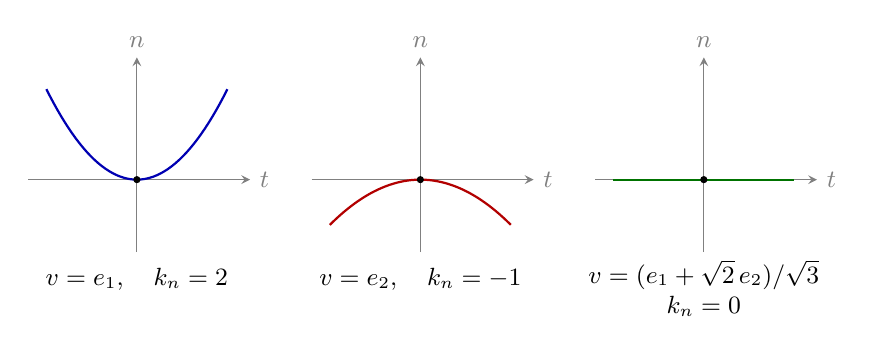
\begin{tikzpicture}[x=1.15cm,y=1.15cm,>=stealth,font=\small]
		\begin{scope}
			\draw[->,gray] (-1.2,0)--(1.25,0) node[right]{\(t\)};
			\draw[->,gray] (0,-0.8)--(0,1.35) node[above]{\(n\)};
			\draw[thick,blue!70!black,domain=-1:1,samples=50] plot(\x,{\x*\x});
			\fill (0,0) circle(1.3pt);
			\node at (0,-1.1){\(v=e_1,\quad k_n=2\)};
		\end{scope}
		\begin{scope}[xshift=3.6cm]
			\draw[->,gray] (-1.2,0)--(1.25,0) node[right]{\(t\)};
			\draw[->,gray] (0,-0.8)--(0,1.35) node[above]{\(n\)};
			\draw[thick,red!70!black,domain=-1:1,samples=50] plot(\x,{-0.5*\x*\x});
			\fill (0,0) circle(1.3pt);
			\node at (0,-1.1){\(v=e_2,\quad k_n=-1\)};
		\end{scope}
		\begin{scope}[xshift=7.2cm]
			\draw[->,gray] (-1.2,0)--(1.25,0) node[right]{\(t\)};
			\draw[->,gray] (0,-0.8)--(0,1.35) node[above]{\(n\)};
			\draw[thick,green!45!black] (-1,0)--(1,0);
			\fill (0,0) circle(1.3pt);
			\node[align=center] at (0,-1.2){\(v=(e_1+\sqrt2\,e_2)/\sqrt3\)\\\(k_n=0\)};
		\end{scope}
	\end{tikzpicture}
	\caption[鞍面在不同方向的法截线]{图像 \(z=x^2-\tfrac12y^2\) 在原点的三条法截线，各自画在由 \(v,n\) 张成的截平面内。三图的横坐标均沿单位切方向 \(v\)，纵坐标沿选定法向 \(n\)；相应截线为 \(z=t^2\)、\(z=-t^2/2\) 与 \(z=0\)。}
	\label{g1:fig:normal-sections}
\end{figure}


\subsection{平均曲率、Gauss 曲率及脐点}
\label{g1:subsec:0802:03}

两个主曲率交换编号时，和与积都不改变。把它们用于刻画曲面，可以避免不断选择和排列主方向。和反映两个正交方向的平均弯曲，积则区分同向弯曲、反向弯曲与二阶退化。

\begin{definition}[平均曲率、Gauss 曲率与脐点]\label{g1:def:surface-curvatures}
	在带选定单位法向的光滑浸入曲面上，定义\term[pingjunqulv]{平均曲率}[mean curvature]与\term[Gaussqulv]{Gauss 曲率}[Gaussian curvature]为
	\[
		H\coloneqq\tfrac12\operatorname{tr}S=\tfrac12(k_1+k_2),\qquad K\coloneqq\det S=k_1k_2.
	\]
	若某点 \(k_1=k_2\)，则称为\term[qidian]{脐点}[umbilic point]，等价地，该点 \(S=HI\)。若 \(S=0\)，称其为\term[pingdian]{平点}[planar point]；平点是两个主曲率都为零的脐点。
	\symidx{\(H\)：平均曲率}
	\symidx{\(K\)：曲面的 Gauss 曲率}
\end{definition}

这里的 \(1/2\) 属于平均曲率的约定，有些文献把主曲率之和直接叫作平均曲率。我们后续的公式均使用上面的平均值。Gauss 曲率目前是通过曲面在三维空间中的法向变化定义的；它是否也能仅由第一基本形式恢复，是下一节要证明的问题。

\begin{proposition}[曲率的计算与法向选择]\label{g1:prop:surface-curvature-formulas}
	设 \(X:U\to\mathbb R^3\) 是光滑浸入，选定单位法向，并使用第一、第二基本形式的系数 \(E,F,G,h_{ij}\)。则
	\begin{equation}\label{g1:eq:surface-HK-formulas}
		K=\frac{h_{11}h_{22}-h_{12}^2}{D},\qquad
		H=\frac{Gh_{11}-2Fh_{12}+Eh_{22}}{2D},\qquad D=EG-F^2.
	\end{equation}
	有 \(H^2-K\ge0\)，两个主曲率是 \(H\pm\sqrt{H^2-K}\)，脐点恰由 \(H^2=K\) 刻画。把法向改为 \(-n\) 时，\(S,\mathrm{II},H\) 同时变号，两个主曲率各自变号，\(K\) 与主方向不变。
\end{proposition}
\begin{proof}
	由\eqref{g1:eq:shape-matrix}，
	\[
		[S]=\frac1D
		\begin{pmatrix}
			Gh_{11}-Fh_{12}&Gh_{12}-Fh_{22}\\
			Eh_{12}-Fh_{11}&Eh_{22}-Fh_{12}
		\end{pmatrix}.
	\]
	取行列式和迹即得\eqref{g1:eq:surface-HK-formulas}。又
	\[
		H^2-K=\tfrac14(k_1-k_2)^2,\qquad
		\det(\lambda I-S)=\lambda^2-2H\lambda+K,
	\]
	所以平方根为实数，二次方程的根给出主曲率，等根恰为脐点。法向翻转后 \(S=-\mathrm dn\) 变号，其余各项由定义得到；若主曲率原先按大小排序，翻转后还须交换顺序。
\end{proof}

例如，外向法向的半径 \(R\) 球面处处有 \(H=-1/R\)、\(K=1/R^2\)，且每一点都是脐点。平面取任一固定单位法向则有 \(S=0\)。与此不同，图像 \(z=x^3-3xy^2\) 只在原点有二阶偏导全部为零，所以原点是平点；在其余位置，二阶偏导矩阵的行列式为 \(-36(x^2+y^2)\)，由图像公式及\eqref{g1:eq:surface-HK-formulas}知 \(K<0\)。因此“一点的第二基本形式为零”不意味着附近的曲面是一张平面。

\ProseParagraphBreak

平均曲率还真的是各方向法曲率的角平均。由 Euler 公式，
\[
	\frac1{2\pi}\int_0^{2\pi}k_n(\cos\theta\,e_1+\sin\theta\,e_2)\,\mathrm d\theta
	=\frac{k_1+k_2}2=H.
\]
平均值为零时，各方向的弯曲可能恰好抵消，不能据此断言每个方向都不弯曲。例如上一小节的鞍面若改为 \(z=x^2-y^2\)，则原点 \(H=0\) 而 \(K=-4\)。

\subsection{曲率线、渐近线及其退化}
\label{g1:subsec:0802:04}

一点上的方向能否沿曲面连成曲线，是另一个问题。先规定要沿哪些方向行走，再讨论方向能否光滑选取以及微分方程是否有解；这两步在脐点或曲率变号处都可能发生变化。

\begin{definition}[曲率线与渐近线]\label{g1:def:principal-asymptotic-curves}
	在带选定单位法向的光滑浸入曲面上，若一条光滑正则曲线的切向量处处为形算子的特征向量，称其为\term[qulvxian]{曲率线}[line of curvature]。若非零切向量 \(v\) 满足 \(\mathrm{II}(v,v)=0\)，称它张成的无向直线为\term[jianjinfangxiang]{渐近方向}[asymptotic direction]；切向量处处为渐近方向的光滑正则曲线称为\term[jianjinxian]{渐近线}[asymptotic curve]。
\end{definition}

法向翻转不改变特征方向，也不改变 \(\mathrm{II}(v,v)=0\) 的解，因此这两类曲线可以不依赖整体法向选择来讨论。曲率线要求法向变化 \(\mathrm dn(v)\) 与行进方向平行；渐近线要求曲线的法向加速度为零。两者是不同条件。

\begin{lemma}[局部积分曲线]\label{g1:lem:surface-field-integral-curve}
	设 \(V:U\to\mathbb R^2\) 是开集 \(U\subset\mathbb R^2\) 上的光滑向量场，\(u_0\in U\)。则在某个 \((-\varepsilon,\varepsilon)\) 上，初值问题
	\[
		\dot u(t)=V(u(t)),\qquad u(0)=u_0
	\]
	有唯一的局部光滑解。若 \(V(u_0)\ne0\)，缩小区间后该解正则。
\end{lemma}
\begin{proof}
	取闭球 \(\overline B(u_0,r)\subset U\)。由于 \(V\) 及其一阶导数在闭球上有界，存在常数 \(M,L\ge0\)，使 \(\lVert V\rVert\le M\) 且 \(\lVert V(x)-V(y)\rVert\le L\lVert x-y\rVert\)。选 \(a>0\) 足够小，使 \(aM<r\)、\(q=aL<1\)。在所有取值于此闭球的连续路径 \(u:[-a,a]\to\overline B(u_0,r)\) 上定义
	\[
		(\mathcal Tu)(t)=u_0+\int_0^t V(u(s))\,\mathrm ds.
	\]
	估计 \(aM<r\) 保证 \(\mathcal T\) 仍取值于闭球，而一致范数满足
	\[
		\lVert\mathcal Tu-\mathcal Tw\rVert_\infty\le q\lVert u-w\rVert_\infty.
	\]
	从常路径 \(u_0\) 迭代 \(u_{m+1}=\mathcal Tu_m\)，相邻两次的差至多按 \(q^m\) 衰减。几何级数收敛说明 \(u_m\) 一致收敛；连续路径的一致极限仍连续且取值于闭球。把极限送入积分，得到 \(u=\mathcal Tu\)，所以 \(u\) 为 \(C^1\) 且满足方程。若 \(u,w\) 都是这个积分方程的解，同一估计给出 \(\lVert u-w\rVert_\infty\le q\lVert u-w\rVert_\infty\)，因而两者相同。任意另一局部解在足够短的公共区间内也留在闭球中，这就给出局部唯一性。由 \(\dot u=V(u)\) 逐次求导，\(u\) 为光滑；最后用 \(V(u_0)\ne0\) 及连续性保证附近速度不消失。
\end{proof}

\begin{proposition}[主方向与渐近方向的局部曲线]\label{g1:prop:principal-asymptotic-lines}
	设 \(X:U\to\mathbb R^3\) 为光滑浸入。
	\begin{enumerate}
		\item 每个非脐点附近有两族局部曲率线；经过给定点、沿指定主方向的局部曲率线唯一到正则重参数化为止。
		\item 每个 \(K<0\) 的点附近有两族局部渐近线；经过给定点、沿指定渐近方向的局部渐近线唯一到正则重参数化为止。
		\item 在一点，若 \(K>0\)，没有渐近方向；若 \(K<0\)，有两条不同的渐近方向；若 \(K=0\) 且 \(S\ne0\)，恰有一条渐近方向，为 \(\ker S\)；若 \(S=0\)，所有方向都是渐近方向。
	\end{enumerate}
\end{proposition}
\begin{proof}
	在非脐点附近，\(H^2-K>0\)。所以
	\[
		k_+=H+\sqrt{H^2-K},\qquad k_-=H-\sqrt{H^2-K}
	\]
	是光滑的不同特征值。相应的线性算子
	\[
		P_+=\frac{S-k_-I}{k_+-k_-},\qquad P_-=\frac{S-k_+I}{k_--k_+}
	\]
	分别投影到两条特征直线上。先取一个光滑切向量场 \(W\)，使 \(P_+W\) 在指定点不为零；例如把该点的一个特征向量按坐标基用常系数延伸。缩小邻域后 \(P_+W\) 始终不为零，归一化得到光滑单位特征向量场 \(e_+\)。同理得到 \(e_-\)，并可按需要调整其符号。把 \(e_+\) 在 \(X_1,X_2\) 下的系数看作 \(U\) 上的非零光滑向量场，应用\cref{g1:lem:surface-field-integral-curve}并复合 \(X\)，即得所需曲率线。另一主方向同样处理。任意沿同一方向的正则曲线，缩短后可调整方向并改用弧长，使其导数等于所选单位场；初值唯一性就给出无参数轨迹的唯一性。

	当 \(K<0\) 时，\(k_+>0>k_-\)。在上面选出的光滑正交单位场中，二次型的零方向由
	\[
		k_+a^2+k_-b^2=0
	\]
	确定，分别由两个光滑非零场
	\[
		\sqrt{-k_-}\,e_++\sqrt{k_+}\,e_-,
		\qquad
		\sqrt{-k_-}\,e_+-\sqrt{k_+}\,e_-
	\]
	张成。归一化后再次应用局部积分曲线引理，得到存在与唯一性。

	最后，在任一点用主方向正交基把 \(\mathrm{II}\) 写成 \(k_1a^2+k_2b^2\)。若两系数同号，此式对非零向量不为零；若异号，得到上面的两条直线；若恰有一个系数为零，解是一条坐标轴；若两者都为零，每个向量都是解。这证明了第三项。
\end{proof}

这份分类只需解一个二元二次方程，可整理为\cref{g1:tab:asymptotic-directions}。其中 \(K=0\) 的两行必须分开：仅凭 \(K\) 的值，无法判断零方向是一条还是所有方向。

\begin{table}[htbp]
	\centering
	\caption{第二基本形式与渐近方向}
	\label{g1:tab:asymptotic-directions}
	\begin{tabular}{lll}
		\toprule
		条件 & 主方向基下的二次型 & 渐近方向 \\
		\midrule
		\(K>0\) & 两个非零系数同号 & 无 \\
		\(K<0\) & 两个系数异号 & 两条不同直线 \\
		\(K=0,\ S\ne0\) & 恰有一个系数为零 & 一条直线 \\
		\(S=0\) & 零二次型 & 所有方向 \\
		\bottomrule
	\end{tabular}
\end{table}

在一整片 \(K=0,\ S\ne0\) 的区域上，零特征值与另一个特征值仍然分离，上面的投影构造同样给出一条光滑方向场及其积分曲线。但若只知道某一点 \(K=0\)，不能据此断言有渐近线穿过它。例如 \(z=x^2+y^4\) 在原点的形算子为 \(\operatorname{diag}(2,0)\)，只有 \(y\) 轴方向渐近；在 \(y\ne0\) 处却有 \(K>0\)，不存在渐近方向。若有正则渐近线通过原点，其速度必须沿 \(y\) 轴且不为零，于是附近离开原点后 \(y\ne0\)，矛盾。因此原点的渐近方向不能延续成穿过该点的渐近线。

\ProseParagraphBreak

脐点处的困难则是主方向不再分离。球面的每条正则曲线都是曲率线，经过一点和一条切向的曲线远不唯一。即使避开脐点，在一张较大的曲面上也不能从局部单位特征向量的选择自动得到全局连续选择：沿闭路延伸后，向量可能反向，而它张成的直线仍相同。曲率线和渐近线的定义使用无向直线，正是为了把这种方向选择与曲线本身区别开。

% !TeX root = ../../Book1.tex
% 纲要标题：### 8.3 结构方程与内在曲率
% 纲要位置：几何学计划纲要.md，第 416 行。
% 正文状态：初稿；尚未正式审核。

% 纲要内容开始
% 
% * Gauss–Weingarten 方程
% * 协变导数与 Christoffel 系数
% * Gauss 方程与绝妙定理
% * Codazzi 方程及混合偏导相容性
% 
% 纲要内容结束

\section{结构方程与内在曲率}
\label{g1:sec:0803}

第一基本形式记录切平面中的长度，第二基本形式记录曲面向法向弯曲的程度。它们看起来各管一件事，但不能任意指定：如果它们来自同一个位置函数 \(X(u,v)\)，先对 \(u\) 求导再对 \(v\) 求导，必须与相反的顺序得到相同结果。这一简单要求将同时给出 Gauss 方程和 Codazzi 方程。Gauss 方程还将把主曲率的乘积写成第一基本形式及其导数的表达式，将法向弯曲与内在度量联系起来。

\ProseParagraphBreak

本节取光滑浸入 \(X\colon U\rightarrow\mathbb R^3\)，其中 \(U\subseteq\mathbb R^2\) 开，记 \(u^1=u\)、\(u^2=v\)、\(X_i=\partial_iX\)。沿用 \(g_{ij}=\langle X_i,X_j\rangle\)、\(D=\det(g_{ij})>0\) 与选定的单位法向 \(n\)，并记 \(h_{ij}=\langle X_{ij},n\rangle\)。向量场及其导数都按参数点定义；若像有自交，不把不同参数点上的切向量混为一谈。指标 \(i,j,k,\ell,m\) 均取 \(1,2\)；在同一项中重复出现的一上一下指标表示对这两个值求和。这个简写只省去求和号，不改变矩阵的乘法顺序。

\subsection{Gauss–Weingarten 方程}
\label{g1:subsec:0803:01}

前一节已经把 \(X_{ij}\) 的法向分量写成 \(h_{ij}n\)。剩下的切向分量也需要记录，因为坐标向量 \(X_1,X_2\) 一般随位置改变，既不保持长度，也不保持夹角。令 \((g^{ij})\) 为 \((g_{ij})\) 的逆矩阵，并写 \(h_i{}^k=g^{k\ell}h_{i\ell}\)。

\begin{proposition}[Gauss–Weingarten 方程]
	\label{g1:prop:gauss-weingarten}
	设 \(U\subseteq\mathbb R^2\) 开，\(X:U\rightarrow\mathbb R^3\) 是光滑浸入，\(n\) 为光滑单位法向。记 \(X_i=\partial_iX\)、\(g_{ij}=\langle X_i,X_j\rangle\)、\(h_{ij}=\langle\partial_i\partial_jX,n\rangle\)、\((g^{ij})=(g_{ij})^{-1}\)，并令 \(h_i{}^k=\sum_\ell g^{k\ell}h_{i\ell}\)。重复指标取 \(1,2\) 并求和。存在唯一的光滑函数 \(\Gamma^k_{ij}\)，使
	\begin{equation}
		\label{g1:eq:gauss-weingarten}
		\partial_iX_j=\Gamma^k_{ij}X_k+h_{ij}n,\qquad
		\partial_i n=-h_i{}^kX_k.
	\end{equation}
	其中 \(\Gamma^k_{ij}=\Gamma^k_{ji}\)，并且
	\begin{equation}
		\label{g1:eq:christoffel-metric}
		\Gamma^k_{ij}
		=\frac12g^{k\ell}\bigl(\partial_i g_{j\ell}+\partial_j g_{i\ell}-\partial_\ell g_{ij}\bigr).
	\end{equation}
	因此 \(X_{ij}\) 的切向分解系数完全由第一基本形式决定。
\end{proposition}

\begin{proof}
	浸入条件保证 \(X_1,X_2,n\) 线性无关，所以向量 \(X_{ij}\) 有唯一的上述分解。混合偏导相等给出 \(\Gamma^k_{ij}=\Gamma^k_{ji}\)。对 \(g_{j\ell}=\langle X_j,X_\ell\rangle\) 求导，得到
	\[
		\partial_i g_{j\ell}=\langle X_{ij},X_\ell\rangle+\langle X_j,X_{i\ell}\rangle.
	\]
	把交换 \(i,j,\ell\) 所得的三个式子按前两个相加、第三个相减，交叉项抵消，故
	\[
		2\langle X_{ij},X_\ell\rangle
		=\partial_i g_{j\ell}+\partial_j g_{i\ell}-\partial_\ell g_{ij}
		=2\Gamma^k_{ij}g_{k\ell}.
	\]
	乘逆矩阵便得\eqref{g1:eq:christoffel-metric}。

	由 \(\langle n,n\rangle=1\) 可知 \(\partial_i n\) 是切向量；对 \(\langle n,X_j\rangle=0\) 求导，又有
	\[
		\langle\partial_i n,X_j\rangle=-\langle n,X_{ij}\rangle=-h_{ij}.
	\]
	若 \(\partial_i n=a^kX_k\)，则 \(a^kg_{kj}=-h_{ij}\)，即 \(a^k=-g^{k\ell}h_{i\ell}\)。
\end{proof}

\eqref{g1:eq:gauss-weingarten}中的第一式称为 Gauss 公式，第二式称为 Weingarten 公式；两式合称\term[gaussweingartenfangcheng]{Gauss–Weingarten 方程}[Gauss--Weingarten equations]。第二式正是形算子 \(S=-\mathrm{d}n\) 的坐标表达；负号与\cref{g1:def:shape-operator}的约定一致。\footnote{Weingarten，Julius Weingarten（1836--1910），德国数学家，研究曲面等距变形与曲率线。}

\ProseParagraphBreak

这里的标架 \((X_1,X_2,n)\) 通常不是正交单位标架。因此 \(\Gamma^k_{ij}\) 无须像\eqref{g1:eq:frenet-matrix}中的系数矩阵那样斜对称。其作用是补偿坐标基自身的变化；这个变化有些来自曲面的弯曲，有些仅来自选了弯曲的坐标线。

\subsection{协变导数与 Christoffel 系数}
\label{g1:subsec:0803:02}

设 \(V=V^iX_i\) 是沿曲面的光滑切向量场。把它当作取值于 \(\mathbb R^3\) 的函数求导，\(\partial_iV\) 未必仍在切平面内。例如球面上的切向量沿曲线变化时，普通导数可能含有径向分量。如果我们只记录曲面自身的切向变化，就应把普通导数投影回当前切平面。

\begin{definition}
	\label{g1:def:surface-covariant-derivative}
	设 \(U\subseteq\mathbb R^2\) 开，\(X:U\rightarrow\mathbb R^3\) 为光滑浸入，\(X_i=\partial_iX\)，\(V=V^iX_i\)、\(W=W^iX_i\) 为沿 \(X\) 的光滑切向量场，\(f\in C^\infty(U)\)，\(\Gamma^k_{ij}\) 为诱导度量的 Christoffel 系数。定义它沿坐标方向的\term[xiebiandaoshu]{协变导数}[covariant derivative]为
	\[
		\nabla_iV\coloneqq(\partial_iV)^\top
		=\bigl(\partial_iV^k+\Gamma^k_{ij}V^j\bigr)X_k,
	\]
	其中 \({}^\top\) 表示向切平面的正交投影。若 \(W=W^iX_i\)，则定义 \(\nabla_WV=W^i\nabla_iV\)。函数的方向导数记为 \(W(f)=W^i\partial_i f\)。\symidx{\(\nabla_WV\)：切向量场的协变导数}
\end{definition}

上式中的 \(\Gamma^k_{ij}\) 称为\term[christoffelxishu]{Christoffel 系数}[Christoffel symbols]，也称 Christoffel 符号。\footnote{Christoffel，Elwin Bruno Christoffel（1829--1900），德国数学家，研究二次微分形式、张量演算与共形映射。}在这里“协变”所强调的是：重参数化后，计算仍给出同一个切向量，而非要求各个数 \(\Gamma^k_{ij}\) 保持不变。定义中的正交投影及方向导数都是几何操作，已经说明其不依赖坐标；公式中新增的 \(\Gamma^k_{ij}V^j\) 恰好补上了基向量求导的部分。\symidx{\(\Gamma^k_{ij}\)：Christoffel 系数}

\begin{example}[平面也可以有非零的 Christoffel 系数]
	\label{g1:exm:polar-christoffel}
	在平面的极坐标参数 \(X(r,\theta)=(r\cos\theta,r\sin\theta,0)\) 中，取 \(r>0\) 及一个适当的角度区间，有 \(g_{rr}=1\)、\(g_{r\theta}=0\)、\(g_{\theta\theta}=r^2\)。代入\eqref{g1:eq:christoffel-metric}得到仅有的非零系数
	\[
		\Gamma^r_{\theta\theta}=-r,\qquad
		\Gamma^\theta_{r\theta}=\Gamma^\theta_{\theta r}=\frac1r.
	\]
	例如 \(\partial_\theta X_\theta=-rX_r\) 只是平面内的径向加速度，并不意味着平面发生了法向弯曲。在直角坐标下，同一平面的全部 Christoffel 系数都为零。
\end{example}

这种现象说明 \(\Gamma^k_{ij}\) 不是一个张量的分量：如果张量在某组基下全部分量为零，换基后仍应全部为零。更直接地，设新坐标为 \(y^a\)，旧坐标为 \(u^i=u^i(y)\)，对 \(\widetilde X(y)=X(u(y))\) 求两次导数，并比较切向分量，得到
\[
	\widetilde\Gamma^c_{ab}
	=\frac{\partial y^c}{\partial u^k}
	\left(
		\Gamma^k_{ij}\frac{\partial u^i}{\partial y^a}\frac{\partial u^j}{\partial y^b}
		+\frac{\partial^2u^k}{\partial y^a\partial y^b}
	\right).
\]
最后的二阶导数项不是逐点线性换基产生的项。协变导数整体仍然与坐标无关，因为向量分量 \(V^i\) 的导数也发生变化，恰好抵消这项。

\ProseParagraphBreak

为了比较先沿两个方向求导的结果，需要注意：任意两个向量场的方向导数未必可交换。定义它们的\term[xiangliangchangkuohao]{向量场括号}[Lie bracket]为
\[
	[W,V]=\bigl(W^i\partial_iV^k-V^i\partial_iW^k\bigr)X_k.
\]
对每个光滑函数 \(f\)，直接展开可得 \([W,V](f)=W(V(f))-V(W(f))\)，其中二阶偏导项成对抵消。这也给出了括号与坐标无关的含义。这一运算也称为 Lie 括号。\footnote{Lie，Marius Sophus Lie（1842--1899），挪威数学家，创立连续变换群理论，并研究其与微分方程的联系。}特别地，坐标向量场满足 \([X_1,X_2]=0\)；这并不是说作为 \(\mathbb R^3\) 值函数的 \(X_1,X_2\) 是常向量。

\begin{proposition}[切向求导的基本性质]
	\label{g1:prop:surface-connection-properties}
	设 \(U\subseteq\mathbb R^2\) 开，\(X:U\to\mathbb R^3\) 为光滑浸入，\(\nabla_WV\) 由普通方向导数沿 \(W\) 求导后向切平面正交投影得到。此协变导数对向量场可加，且对任意光滑函数 \(f\) 及切向量场 \(V,W,Z\)，有
	\begin{align*}
		\nabla_{fW}V&=f\nabla_WV,&
		\nabla_W(fV)&=W(f)V+f\nabla_WV,\\
		W\langle V,Z\rangle&=\langle\nabla_WV,Z\rangle+\langle V,\nabla_WZ\rangle,&
		\nabla_WV-\nabla_VW&=[W,V].
	\end{align*}
	后两条分别称为\term[duliangxiangrong]{度量相容}[metric compatibility]和\term[wunao]{无挠性}[torsion-freeness]。更一般地，在开集 \(U\subseteq\mathbb R^2\) 上给定任意光滑正定矩阵场 \(g=(g_{ij})\)，令 \((g^{ij})=(g_{ij})^{-1}\)，按 Christoffel 公式\eqref{g1:eq:christoffel-metric}，即 \(\Gamma^k_{ij}=\tfrac12g^{k\ell}(\partial_i g_{j\ell}+\partial_j g_{i\ell}-\partial_\ell g_{ij})\)，及 \(\nabla_WV=W^i(\partial_iV^k+\Gamma^k_{ij}V^j)\partial_k\) 定义的运算也满足这两条性质，而且它是满足这些性质与前两条求导规则的唯一运算。
\end{proposition}

\begin{proof}
	前两条由普通求导的线性及乘法法则得到。对于诱导度量，普通内积求导后出现的法向分量与 \(V,Z\) 垂直，所以投影不改变结果，得到度量相容。再展开 \(\nabla_WV-\nabla_VW\)，由于 \(\Gamma^k_{ij}=\Gamma^k_{ji}\)，所有含 \(\Gamma\) 的项相消，余项就是括号。

	对于任意给定的正定 \(g\)，公式\eqref{g1:eq:christoffel-metric}仍给出 \(\Gamma^k_{ij}=\Gamma^k_{ji}\)，所以无挠性的证明不变。另有
	\[
		\Gamma^k_{ij}g_{k\ell}+\Gamma^k_{i\ell}g_{jk}
		=\partial_i g_{j\ell},
	\]
	因为将右式中的两个 \(\Gamma\) 换成定义后，其余偏导项互相抵消。这正是对坐标向量场的度量相容，乘以向量场分量并用乘法法则即得一般情形。

	最后，设另一运算满足相同规则，写其坐标系数为 \(C^k_{ij}\)。无挠性给出 \(C^k_{ij}=C^k_{ji}\)，度量相容给出 \(\partial_i g_{j\ell}=C^k_{ij}g_{k\ell}+C^k_{i\ell}g_{jk}\)。如\cref{g1:prop:gauss-weingarten}的证明那样将三个式子相加减，就强制得到 \(C^k_{ij}=\Gamma^k_{ij}\)。
\end{proof}

这一运算也称为度量的\term[lianluo]{联络}[connection]。在只给定 \(g\) 而尚未构造曲面时，我们把坐标基写作 \(\partial_1,\partial_2\)，完全可以照同一公式求导。重参数化后，度量相容、无挠性和两条求导规则都保持；上面的唯一性说明，各套坐标得到的是同一个运算。因此，“把普通导数投影回去”是诱导度量的直观构造，“由 \(g\) 的系数求出 \(\Gamma\)”则使这个构造不再依赖于周围的三维空间。

\subsection{Gauss 方程与绝妙定理}
\label{g1:subsec:0803:03}

普通二阶偏导可交换，协变二阶导数却是在每次求导后都投影一次，两次中间使用的切平面不同，结果可能不同。若方向本身也是变化的向量场，还必须扣除它们的括号造成的差别。扣除这一差别后，结果才能只依赖给定点上的方向。

\begin{definition}
	\label{g1:def:surface-curvature-tensor}
	设 \((M,g)\) 为光滑度量曲面，\(\nabla\) 为 \(g\) 的无挠相容协变导数。对任意光滑切向量场 \(V,W,Z\)，定义
	\[
		R(V,W)Z\coloneqq\nabla_V\nabla_WZ-\nabla_W\nabla_VZ-\nabla_{[V,W]}Z.
	\]
	这个运算称为\term[qulvzhangliang]{曲率张量}[curvature tensor]。本书固定上述符号顺序。\symidx{\(R(V,W)Z\)：曲率张量}
\end{definition}

\begin{proposition}
	\label{g1:prop:curvature-tensorial}
	设 \(M\) 为光滑曲面，\(\nabla\) 为其切丛上的光滑联络，\(V,W,Z\) 为光滑切向量场。令 \(R(V,W)Z=\nabla_V\nabla_WZ-\nabla_W\nabla_VZ-\nabla_{[V,W]}Z\)，此处不要求联络无挠或与度量相容。则 \(R(V,W)Z\) 对三个向量场均为逐点线性：任意光滑函数 \(f\) 均满足
	\begin{align*}
		R(fV,W)Z&=fR(V,W)Z,\\
		R(V,fW)Z&=fR(V,W)Z,\\
		R(V,W)(fZ)&=fR(V,W)Z.
	\end{align*}
	因此在点 \(p\) 的值只依赖 \(V(p),W(p),Z(p)\)，不依赖这些向量在邻域中的延拓。
\end{proposition}

\begin{proof}
	先由括号的坐标式得到 \([fV,W]=f[V,W]-W(f)V\)。代入定义，第二项求导产生的 \(-W(f)\nabla_VZ\) 正好与括号项中的 \(W(f)\nabla_VZ\) 抵消，证明第一式。由 \(R(W,V)=-R(V,W)\) 得第二式。

	对第三式，把两次乘法法则代入定义。含 \(\nabla_VZ,\nabla_WZ\) 的一阶导数项成对抵消，剩余的额外项只有
	\[
		\bigl(V(W(f))-W(V(f))-[V,W](f)\bigr)Z=0.
	\]
	故第三式成立。将三个向量场各自在坐标基中展开，所得值是各自分量在 \(p\) 的乘积乘以 \(R(X_i,X_j)X_k\) 在 \(p\) 的值，所以确实只需要三个输入向量的点值。
\end{proof}

这里“张量”的具体含义是：在每一点，这个多线性映射都把三个切向量映为一个切向量。

\ProseParagraphBreak

由于 \([X_1,X_2]=0\)，计算坐标分量只须展开两次求导：
\begin{equation}
	\label{g1:eq:surface-curvature-components}
	\begin{aligned}
		R(X_1,X_2)X_j&=R^k{}_{j12}X_k,\\
		R^k{}_{j12}
		&=\partial_1\Gamma^k_{2j}-\partial_2\Gamma^k_{1j}
		+\Gamma^k_{1m}\Gamma^m_{2j}-\Gamma^k_{2m}\Gamma^m_{1j}.
	\end{aligned}
\end{equation}
例如 \(\nabla_1(\Gamma^m_{2j}X_m)\) 同时对系数及基向量求导，才得到偏导项和两个系数的乘积。遗漏后一部分，就会把坐标基变化误当作曲率。

\begin{theorem}[Gauss 方程]
	\label{g1:thm:gauss-equation}
	设 \(U\subseteq\mathbb R^2\) 开，\(X:U\rightarrow\mathbb R^3\) 是光滑浸入，取光滑单位法向 \(n\)，形算子为 \(S=-\mathrm{d}n\)，第二基本形式为 \(h(V,W)=\langle SV,W\rangle\)。以 \(\nabla\) 记诱导度量的无挠相容协变导数，定义 \(R(V,W)Z=\nabla_V\nabla_WZ-\nabla_W\nabla_VZ-\nabla_{[V,W]}Z\)，其中 \(V,W,Z\) 为光滑切向量场。令 \(X_i=\partial_iX\)、\(g_{ij}=\langle X_i,X_j\rangle\)、\((g^{ij})=(g_{ij})^{-1}\)、\(h_{ij}=h(X_i,X_j)\)、\(h_i{}^k=g^{k\ell}h_{i\ell}\)，并以 \(R(X_1,X_2)X_j=R^k{}_{j12}X_k\) 定义曲率分量。则曲率满足
	\begin{equation}
		\label{g1:eq:gauss-equation}
		R(V,W)Z=h(W,Z)SV-h(V,Z)SW.
	\end{equation}
	特别地，
	\[
		R^k{}_{j12}=h_{2j}h_1{}^k-h_{1j}h_2{}^k,\qquad
		\langle R(X_1,X_2)X_2,X_1\rangle=h_{11}h_{22}-h_{12}^2.
	\]
\end{theorem}

\begin{proof}
	记 \(\mathrm{D}_V\) 为对 \(\mathbb R^3\) 值函数逐分量作方向导数。由定义及\cref{g1:prop:gauss-weingarten}，任意切向量场满足
	\[
		\mathrm{D}_VZ=\nabla_VZ+h(V,Z)n,\qquad \mathrm{D}_Vn=-SV.
	\]
	Euclid 空间中的逐分量求导满足
	\[
		\mathrm{D}_V\mathrm{D}_WZ-\mathrm{D}_W\mathrm{D}_VZ-\mathrm{D}_{[V,W]}Z=0,
	\]
	因为对每个分量这正是括号的定义。将前两个分解式代入，并只取切向分量：
	\[
		0=\nabla_V\nabla_WZ-h(W,Z)SV
		-\nabla_W\nabla_VZ+h(V,Z)SW-\nabla_{[V,W]}Z.
	\]
	移项便得 Gauss 方程。最后取 \(V=X_1,W=Z=X_2\)，再与 \(X_1\) 作内积，使用 \(h(X_i,X_j)=h_{ij}\)，即可得到坐标结论。
\end{proof}

上面的等式称为\term[gaussfangcheng]{Gauss 方程}[Gauss equation]。左边只由度量求导得到，右边却是法向弯曲的数据。由\cref{g1:prop:surface-curvature-formulas}，\(K=\det(h_{ij})/\det(g_{ij})\)，因此立即得到
\begin{equation}
	\label{g1:eq:intrinsic-gauss-curvature}
	K=\frac{\langle R(X_1,X_2)X_2,X_1\rangle}{D}
	=\frac{g_{1k}R^k{}_{212}}{D}.
\end{equation}
其右端只使用 \(g_{ij}\)、它们的逆矩阵和一二阶偏导数。

\begin{theorem}[Gauss 绝妙定理]
	\label{g1:thm:theorema-egregium}
	光滑曲面的 Gauss 曲率由第一基本形式决定。若两个光滑正则曲面片局部等距，则对应点的 Gauss 曲率相等；此结论不要求局部等距来自三维 Euclid 空间的刚性变换，也不要求保持所选法向。
\end{theorem}

\begin{proof}
	设局部等距在参数域中由微分同胚 \(\phi\) 表示。用 \(\phi\) 重参数化第二个曲面片后，它与第一个曲面片的 \(g_{ij}\) 完全相同，因而\eqref{g1:eq:christoffel-metric}给出相同的 \(\Gamma^k_{ij}\)，\eqref{g1:eq:surface-curvature-components}给出相同的 \(R^k{}_{j12}\)。再由\eqref{g1:eq:intrinsic-gauss-curvature}，两者的 \(K\) 相同。反转法向虽使 \(h,S\) 变号，却不改变 \(\det S\)，所以结论也不依赖该选择。
\end{proof}

这一定理称为\term[juemiaodingli]{绝妙定理}[theorema egregium]。内在度量确定两主曲率的乘积；平面与圆柱可以局部等距而主曲率不同，说明单个主曲率还记录着外在弯曲。另一方面，标准球面有 \(K=1/R^2\)，平面有 \(K=0\)，所以球面上任何开片都不能通过保持长度的局部等距完全铺到平面上。

\ProseParagraphBreak

下一节将从给定的度量与对称形式出发，尚无曲面可供求导。为此要明确：二维度量的曲率也只有一个独立的数，因而一个标量 Gauss 方程足以表达全部曲率条件。

\begin{proposition}[二维曲率只有一个独立分量]
	\label{g1:prop:surface-curvature-two-dim}
	设 \(g\) 是开集 \(U\subseteq\mathbb R^2\) 上的光滑正定度量，令 \((g^{ij})=(g_{ij})^{-1}\)，按\eqref{g1:eq:christoffel-metric}，即 \(\Gamma^k_{ij}=\tfrac12g^{k\ell}(\partial_i g_{j\ell}+\partial_jg_{i\ell}-\partial_\ell g_{ij})\)，定义 \(\nabla_i\partial_j=\Gamma^k_{ij}\partial_k\)，并令 \(R(V,W)Z=\nabla_V\nabla_WZ-\nabla_W\nabla_VZ-\nabla_{[V,W]}Z\)。令
	\[
		K_g\coloneqq\frac{g(R(\partial_1,\partial_2)\partial_2,\partial_1)}
		{\det(g_{ij})}.
	\]
	则 \(K_g\) 不依赖坐标，且任意切向量 \(V,W,Z\) 都满足
	\begin{equation}
		\label{g1:eq:two-dimensional-curvature}
		R(V,W)Z=K_g\bigl(g(W,Z)V-g(V,Z)W\bigr).
	\end{equation}
	若另给 \(U\) 上的一个光滑对称双线性形式 \(h\)，令 \(S=g^{-1}h\)，则标量等式 \(K_g=\det S\) 等价于完整的 Gauss 方程\eqref{g1:eq:gauss-equation}。
\end{proposition}

\begin{proof}
	固定一点，令 \(C(V,W,Z,T)=g(R(V,W)Z,T)\)。定义给出 \(C\) 在前两个变量中反对称。度量相容又给出
	\[
		g(R(V,W)Z,T)+g(Z,R(V,W)T)=0.
	\]
	要验证这式，只须对 \(g(Z,T)\) 应用恒等式 \(VW-WV-[V,W]=0\)，每次用度量相容展开；含一次协变导数的交叉内积抵消，剩余的正是这两项。因此 \(C\) 在最后两个变量中也反对称。

	取该点的任意正交单位基 \(e_1,e_2\)。二维空间的交替双线性形式只有一个独立分量：若 \(V=ae_1+be_2\)、\(W=ce_1+de_2\)，则前两个位置按双线性与反对称性展开后只剩系数 \(ad-bc\)。对最后两个位置作同样展开，整个 \(C\) 就由
	\[
		k=C(e_1,e_2,e_2,e_1)
	\]
	决定。具体地，
	\[
		C(V,W,Z,T)=k\bigl(g(W,Z)g(V,T)-g(V,Z)g(W,T)\bigr).
	\]
	取 \(V=\partial_1,W=Z=\partial_2,T=\partial_1\)，括号内是 \(g_{11}g_{22}-g_{12}^2\)，故 \(k=K_g\)，同时得到\eqref{g1:eq:two-dimensional-curvature}。右式也表明，在任意另一组基上用同一比值求出的仍是 \(k\)，所以与坐标无关。

	最后，\(S=g^{-1}h\) 关于 \(g\) 自伴。在一点选取它的正交单位特征基，设特征值为 \(a,b\)。此时直接在基向量上计算可得
	\[
		h(W,Z)SV-h(V,Z)SW
		=ab\bigl(g(W,Z)V-g(V,Z)W\bigr).
	\]
	两边对 \(V,W,Z\) 多线性，因此对任意向量成立。又 \(ab=\det S\)，与已证公式比较便得到等价性。
\end{proof}

这里的 \(K_g\) 可以在尚未证明度量能够浸入 \(\mathbb R^3\) 时定义。若确有这样的浸入，Gauss 方程才把它与外在定义的 \(K=\det S\) 认作同一个函数。这一区别会在给定数据的实现问题中起作用。

\begin{example}[共形坐标中的内在曲率]
	\label{g1:exm:conformal-curvature}
	设在参数域上给定度量
	\[
		g=e^{2\phi(u,v)}(\mathrm du^2+\mathrm dv^2),
	\]
	其中 \(\phi\) 光滑。两坐标方向垂直，且长度按同一倍数缩放。由\eqref{g1:eq:christoffel-metric}，
	\[
		\begin{array}{lll}
			\Gamma^1_{11}=\phi_u,&\Gamma^1_{12}=\Gamma^1_{21}=\phi_v,&\Gamma^1_{22}=-\phi_u,\\
			\Gamma^2_{11}=-\phi_v,&\Gamma^2_{12}=\Gamma^2_{21}=\phi_u,&\Gamma^2_{22}=\phi_v.
		\end{array}
	\]
	计算 \(R^1{}_{212}\) 时，两个乘积和恰好抵消：
	\[
		R^1{}_{212}
		=-\phi_{uu}-\phi_{vv}
		+\bigl(-\phi_u^2+\phi_v^2\bigr)
		-\bigl(\phi_v^2-\phi_u^2\bigr)
		=-\phi_{uu}-\phi_{vv}.
	\]
	由于 \(g_{12}=0\)、\(g_{11}=e^{2\phi}\)、\(D=e^{4\phi}\)，得到
	\begin{equation}
		\label{g1:eq:conformal-gauss-curvature}
		K_g=-e^{-2\phi}(\phi_{uu}+\phi_{vv}).
	\end{equation}
	例如 \(\phi=\log2-\log(1+u^2+v^2)\) 时，\(\phi_{uu}+\phi_{vv}=-4/(1+u^2+v^2)^2\)，故 \(K_g=1\)。求出这个数不需要先构造法向或主曲率。
\end{example}

\subsection{Codazzi 方程及混合偏导相容性}
\label{g1:subsec:0803:04}

Gauss 方程比较的是二阶求导的切向部分。法向部分也必须相等，而其中包含的是 \(h_{ij}\) 的一阶变化。直接比较 \(\partial_1h_{2j}\) 与 \(\partial_2h_{1j}\) 还不够，因为 \(h\) 的两个输入基向量也随位置改变，需要把这两种变化扣除。

\begin{definition}
	\label{g1:def:covariant-h-derivative}
	设 \((M,g)\) 为光滑度量曲面，\(\nabla\) 为其无挠相容协变导数，\(h\) 为 \(M\) 上的光滑对称双线性形式。对光滑切向量场 \(V,W,Z\)，定义
	\[
		(\nabla_Vh)(W,Z)
		\coloneqq V\bigl(h(W,Z)\bigr)-h(\nabla_VW,Z)-h(W,\nabla_VZ).
	\]
	在局部坐标中，令 \(h_{jk}=h(\partial_j,\partial_k)\)、\(\nabla_i\partial_j=\Gamma^m_{ij}\partial_m\)，其坐标分量记为
	\[
		\nabla_i h_{jk}\coloneqq\partial_i h_{jk}
		-\Gamma^m_{ij}h_{mk}-\Gamma^m_{ik}h_{jm}.
	\]
\end{definition}

这个定义中的两个减项分别对应 \(h\) 的两个输入。利用协变导数的乘法法则可以检查：将 \(W\) 或 \(Z\) 换成 \(fW\) 或 \(fZ\)，求导产生的 \(V(f)\) 项被相应减项抵消；对 \(V\) 则直接逐点线性。因此 \(\nabla h\) 的值同样不依赖输入向量场的延拓。

\begin{theorem}[Codazzi 方程]
	\label{g1:thm:codazzi-equation}
	设 \(U\subseteq\mathbb R^2\) 开，\(X:U\rightarrow\mathbb R^3\) 是光滑浸入，\(n\) 为光滑单位法向，\(h\) 为相应第二基本形式，\(S=-\mathrm{d}n\) 为形算子，\(\nabla\) 为诱导度量的无挠相容协变导数，则
	\[
		(\nabla_Vh)(W,Z)=(\nabla_Wh)(V,Z)
	\]
	对任意光滑切向量场 \(V,W,Z\) 成立。在局部坐标中，令 \(h_{ij}=h(\partial_i,\partial_j)\)、\(\nabla_i\partial_j=\Gamma^m_{ij}\partial_m\)，坐标表达为两个方程
	\begin{equation}
		\label{g1:eq:codazzi-components}
		\nabla_1h_{2j}-\nabla_2h_{1j}
		=\partial_1h_{2j}-\partial_2h_{1j}
		+\Gamma^m_{2j}h_{1m}-\Gamma^m_{1j}h_{2m}=0,
		\qquad j=1,2.
	\end{equation}
	若定义 \((\nabla_VS)W=\nabla_V(SW)-S(\nabla_VW)\)，则同一条件也可写成 \((\nabla_VS)W=(\nabla_WS)V\)。
\end{theorem}

\begin{proof}
	对 Gauss–Weingarten 方程求一次偏导。由于 \(\partial_i n\) 与 \(n\) 垂直，
	\[
		\langle\partial_1\partial_2X_j,n\rangle
		=\Gamma^m_{2j}h_{1m}+\partial_1h_{2j},\qquad
		\langle\partial_2\partial_1X_j,n\rangle
		=\Gamma^m_{1j}h_{2m}+\partial_2h_{1j}.
	\]
	混合偏导相等立即给出\eqref{g1:eq:codazzi-components}。它与协变导数的表达相同，是因为展开 \(\nabla_1h_{2j}-\nabla_2h_{1j}\) 后，项 \(-\Gamma^m_{12}h_{mj}\) 与 \(+\Gamma^m_{21}h_{mj}\) 相消。其余恰为上式。前面已经证明 \(\nabla h\) 对三个输入逐点线性，所以在坐标基上验证便给出一般向量场的结论。

	最后，度量相容以及 \(h(W,Z)=g(SW,Z)\) 给出
	\[
		(\nabla_Vh)(W,Z)
		=g\bigl(\nabla_V(SW)-S(\nabla_VW),Z\bigr).
	\]
	因度量非退化，对所有 \(Z\) 的内积相等当且仅当对应向量相等，这就得到形算子形式。
\end{proof}

这些关系称为\term[codazzifangcheng]{Codazzi 方程}[Codazzi equations]。\footnote{Codazzi，Delfino Codazzi（1824--1873），意大利数学家，研究曲面基本形式的相容关系与曲线坐标。}它们控制第二基本形式沿不同方向的变化，Gauss 方程则控制第二基本形式与度量曲率的对应。把两种分量放回同一次计算，可直接看见它们的共同来源：
\begin{equation}
	\label{g1:eq:mixed-surface-derivatives}
	\begin{aligned}
		0&=\partial_1\partial_2X_j-\partial_2\partial_1X_j\\
		&=\bigl(R^k{}_{j12}-h_{2j}h_1{}^k+h_{1j}h_2{}^k\bigr)X_k
		+\bigl(\nabla_1h_{2j}-\nabla_2h_{1j}\bigr)n.
	\end{aligned}
\end{equation}
这里切向与法向线性无关，所以两类系数必须分别消失。对于已经存在的曲面，这给出了必要条件；下一节将反过来证明，在足够小的参数邻域内，这些条件也足以从 \(g\) 与 \(h\) 恢复曲面。

% !TeX root = ../../Book1.tex
% 纲要标题：### 8.4 曲面基本定理的连续证明
% 纲要位置：几何学计划纲要.md，第 423 行。
% 正文状态：初稿；尚未正式审核。

% 纲要内容开始
% 
% * 相容数据的矩阵组织
% 
%   把第一、第二基本形式转写成带正交约束的标架系统，确认正定性及法向约定。
% 
% * Gauss–Codazzi 与平坦性
% 
%   计算结构方程，逐项识别给定条件恰好消除混合偏导障碍。
% 
% * 相容一阶系统的局部解
% 
%   建立本章所需的积分引理；不能以尚未证明的一般 Frobenius 定理替代。
% 
% * 从标架到闭的向量值一形式
% 
%   以第一基本形式组装待积分的微分，证明其外微分为零。
% 
% * 浸入的构造和秩检验
% 
%   积分得到位置向量，并用正定性证明微分秩为二。
% 
% * 两基本形式的恢复
% 
%   逐项核对所得浸入的度量和第二基本形式。
% 
% * 局部唯一性与整体单值
% 
%   比较两个标架初值；局部相差刚性变换，非单连通区域另有运输障碍。
% 
% 纲要内容结束

\section{曲面基本定理的连续证明}
\label{g1:sec:0804}

上一节由已经存在的曲面导出了相容条件。本节反过来：给定长度数据 \(g_{ij}\) 和弯曲数据 \(h_{ij}\)，若它们满足那些条件，是否确有一个曲面实现它们？第七章恢复曲线时只需沿一个参数积分标架；曲面有两个参数，沿不同方向走到同一点必须得到相同结果。因而这里真正增加的困难是两组微分方程能否同时成立。我们先把这个困难归结为一个矩阵恒等式，再用两次普通积分解决它。

\subsection{相容数据的矩阵组织}
\label{g1:subsec:0804:01}

设 \(U\subseteq\mathbb R^2\) 为开集，坐标记为 \(u^1=u,\ u^2=v\)，给定光滑函数 \(g_{ij}=g_{ji}\) 和 \(h_{ij}=h_{ji}\)，其中矩阵 \(g=(g_{ij})\) 处处正定。这里的“光滑”指 \(C^\infty\)。记
\[
	g=\begin{pmatrix}E&F\\F&G\end{pmatrix},\qquad D=EG-F^2>0,
	\qquad h_i{}^k=\sum_{\ell=1}^2g^{k\ell}h_{i\ell}.
\]
由 \(g\) 按\eqref{g1:eq:christoffel-metric}计算 \(\Gamma^k_{ij}\)。暂时还没有曲面，因而 \(\Gamma^k_{ij}\) 只是由给定函数计算出的函数。\cref{g1:prop:surface-connection-properties}的证明只用了 \(g\) 的正定性和这个公式，故其无挠条件 \(\Gamma^k_{ij}=\Gamma^k_{ji}\) 与度量相容等式在这里仍然成立。

\ProseParagraphBreak

假如曲面已经存在，它的三个列向量 \(\mathcal F=(X_u,X_v,n)\) 应满足 Gauss–Weingarten 方程。照\eqref{g1:eq:gauss-weingarten}把各列的系数排列起来，就得到待求系统
\begin{equation}
	\label{g1:eq:surface-coordinate-frame-system}
	\partial_i\mathcal F=\mathcal F A_i,\qquad
	A_i=
	\begin{pmatrix}
		\Gamma^1_{i1}&\Gamma^1_{i2}&-h_i{}^1\\
		\Gamma^2_{i1}&\Gamma^2_{i2}&-h_i{}^2\\
		h_{i1}&h_{i2}&0
	\end{pmatrix},\quad i=1,2.
\end{equation}
乘法仍在右边：例如第三列规定 \(\partial_i n=-h_i{}^1X_u-h_i{}^2X_v\)。与曲线的 Frenet 标架不同，\(X_u,X_v\) 通常既不单位也不垂直。因此这里要保持的不是 \(\mathcal F^{\mathsf T}\mathcal F=I\)，而是
\[
	\mathcal F^{\mathsf T}\mathcal F=\mathcal G,\qquad
	\mathcal G=\begin{pmatrix}E&F&0\\F&G&0\\0&0&1\end{pmatrix}.
\]
度量相容性和 \(h_{ij}=h_{ji}\) 给出
\begin{equation}
	\label{g1:eq:surface-matrix-metric-compatibility}
	\partial_i\mathcal G=A_i^{\mathsf T}\mathcal G+\mathcal G A_i.
\end{equation}
左上角的等式就是 \(\partial_i g_{jk}=\Gamma^\ell_{ij}g_{\ell k}+\Gamma^\ell_{ik}g_{j\ell}\)，右上角则是 \(h_{ij}-g_{j\ell}h_i{}^\ell=0\)，其余各块由转置或 \(0=0\) 得到。本节沿用上一节的求和约定：同一项中重复的一上一下指标从 \(1\) 到 \(2\) 求和。

\ProseParagraphBreak

为了直接使用正交标架的积分办法，先把给定长度拆出来。取
\begin{equation}
	\label{g1:eq:surface-metric-factor}
	P=
	\begin{pmatrix}
		\sqrt E&F/\sqrt E&0\\
		0&\sqrt D/\sqrt E&0\\
		0&0&1
	\end{pmatrix}.
\end{equation}
由于 \(E,D>0\)，它光滑、可逆，且 \(P^{\mathsf T}P=\mathcal G\)、\(\det P=\sqrt D>0\)。若令 \(\mathcal F=WP\)，所求三个向量就写成
\[
	a_1=\sqrt E\,e_1,\qquad
	a_2=\frac F{\sqrt E}e_1+\frac{\sqrt D}{\sqrt E}e_2,\qquad
	n=e_3,
\]
其中 \(W=(e_1,e_2,e_3)\) 是右手正交标架。这正是按给定长度和夹角拼出两个切向量；正平方根保证 \(a_1\times a_2=\sqrt D\,n\)，同时固定法向约定。

\ProseParagraphBreak

将 \(\mathcal F=WP\) 代入\eqref{g1:eq:surface-coordinate-frame-system}，可知只需解
\begin{equation}
	\label{g1:eq:surface-orthonormal-frame-system}
	\partial_iW=W\Omega_i,\qquad
	\Omega_i=(PA_i-\partial_iP)P^{-1}.
\end{equation}
这些系数确实斜对称。事实上，由\eqref{g1:eq:surface-matrix-metric-compatibility}，
\[
	P^{\mathsf T}(\Omega_i^{\mathsf T}+\Omega_i)P
	=A_i^{\mathsf T}\mathcal G+\mathcal G A_i-\partial_i(P^{\mathsf T}P)=0.
\]
因 \(P\) 可逆，故 \(\Omega_i^{\mathsf T}=-\Omega_i\)。至此，给定的非正交长度约束已变成一个正交标架系统。

\subsection{Gauss–Codazzi 与平坦性}
\label{g1:subsec:0804:02}

若可逆矩阵函数 \(\mathcal F\) 满足两组方程，交换混合偏导得到
\[
	0=\partial_1\partial_2\mathcal F-\partial_2\partial_1\mathcal F
	=\mathcal F\bigl(\partial_1A_2-\partial_2A_1+A_1A_2-A_2A_1\bigr).
\]
因此括号内的矩阵必须为零。对于一个矩阵系统，条件
\begin{equation}
	\label{g1:eq:surface-flatness}
	\mathcal C\coloneqq\partial_1A_2-\partial_2A_1+[A_1,A_2]=0,
	\qquad [A_1,A_2]=A_1A_2-A_2A_1
\end{equation}
称为该系统的\term[pingtanxing]{平坦性}[flatness]。这个名称指三个标架向量的整体运输方程，不是说给定曲面一定有 \(K=0\)；曲面的内在曲率和法向弯曲可以在 \(\mathcal C\) 中恰好抵消。

\begin{proposition}[相容条件与矩阵平坦性]
	\label{g1:prop:surface-data-flatness}
	设 \(g\) 是平面开集 \(U\) 上的光滑正定对称矩阵，\(h\) 是光滑对称矩阵，各矩阵均为 \(2\times2\)。令 \(D=\det g\)、\((g^{ij})=g^{-1}\)、\(h_i{}^k=g^{k\ell}h_{i\ell}\)，\(\Gamma\) 由 \(g\) 的 Christoffel 公式确定。对 \(i=1,2\)，令 \(A_i=\begin{psmallmatrix}\Gamma^1_{i1}&\Gamma^1_{i2}&-h_i{}^1\\\Gamma^2_{i1}&\Gamma^2_{i2}&-h_i{}^2\\h_{i1}&h_{i2}&0\end{psmallmatrix}\)，即\eqref{g1:eq:surface-coordinate-frame-system}中的系数矩阵，并令 \(\mathcal C=\partial_1A_2-\partial_2A_1+A_1A_2-A_2A_1\)。则 \(\mathcal C=0\) 等价于 Gauss、Codazzi 两组分量等式
	\begin{align}
		\label{g1:eq:surface-data-gauss}
		R^k{}_{j12}&=h_1{}^kh_{2j}-h_2{}^kh_{1j},&&j,k=1,2,\\
		\label{g1:eq:surface-data-codazzi}
		\nabla_1h_{2j}&=\nabla_2h_{1j},&&j=1,2.
	\end{align}
	其中 \(R\) 是 \(\nabla_i\partial_j=\Gamma^k_{ij}\partial_k\) 的曲率，约定 \(R(V,W)Z=\nabla_V\nabla_WZ-\nabla_W\nabla_VZ-\nabla_{[V,W]}Z\)，并以 \(R(\partial_1,\partial_2)\partial_j=R^k{}_{j12}\partial_k\) 定义分量，按\eqref{g1:eq:surface-curvature-components}计算；\(\nabla_i h_{jk}=\partial_i h_{jk}-\Gamma^\ell_{ij}h_{\ell k}-\Gamma^\ell_{ik}h_{j\ell}\)。等价地，第一组条件可以换成 \(K_g=(h_{11}h_{22}-h_{12}^2)/D\)，其中 \(K_g=\langle R(\partial_u,\partial_v)\partial_v,\partial_u\rangle_g/D\) 完全由 \(g\) 决定。
\end{proposition}

\begin{proof}
	按前两行与最后一行分块。矩阵 \(\mathcal C\) 左上角的第 \(k,j\) 项为
	\[
		\partial_1\Gamma^k_{2j}-\partial_2\Gamma^k_{1j}
		+\Gamma^k_{1\ell}\Gamma^\ell_{2j}-\Gamma^k_{2\ell}\Gamma^\ell_{1j}
		-h_1{}^kh_{2j}+h_2{}^kh_{1j}.
	\]
	前四项正是 \(R^k{}_{j12}\)，故这一块消失恰好等价于 Gauss 方程。左下角的第 \(j\) 项为
	\[
		\partial_1h_{2j}-\partial_2h_{1j}
		+h_{1\ell}\Gamma^\ell_{2j}-h_{2\ell}\Gamma^\ell_{1j}
		=\nabla_1h_{2j}-\nabla_2h_{1j}.
	\]
	最后一步中另外两项 \(-\Gamma^\ell_{12}h_{\ell j}\) 与 \(+\Gamma^\ell_{21}h_{\ell j}\) 因无挠条件抵消。右下角是 \(-h_{1\ell}h_2{}^\ell+h_{2\ell}h_1{}^\ell=0\)，因为 \(g^{-1}\) 对称。

	还需检查右上角，不能仅凭矩阵对称性猜测它。交换\eqref{g1:eq:surface-matrix-metric-compatibility}的混合偏导并代回同一等式，展开后得到
	\[
		\mathcal C^{\mathsf T}\mathcal G+\mathcal G\mathcal C=0.
	\]
	当左上角和左下角已为零时，写 \(\mathcal C=\left(\begin{smallmatrix}0&b\\0&0\end{smallmatrix}\right)\)，上式的右上角便是 \(gb=0\)。正定矩阵 \(g\) 可逆，所以 \(b=0\)。这证明两组几何条件足以使整个 \(\mathcal C\) 消失；反向则直接读取上述两块。

	最后，\cref{g1:prop:surface-curvature-two-dim}已对任意光滑正定 \(g\) 证明，二维曲率张量由 \(\langle R(\partial_u,\partial_v)\partial_v,\partial_u\rangle_g\) 这一分量确定。Gauss 方程右边也有相同的交替性和度量斜对称性；其这一分量为 \(h_{11}h_{22}-h_{12}^2\)。故完整的 Gauss 分量条件与所述标量条件等价。
\end{proof}

换成正交标架不会增加新的相容条件。用 \(\partial_iP^{-1}=-P^{-1}(\partial_iP)P^{-1}\) 展开\eqref{g1:eq:surface-orthonormal-frame-system}，可以把二阶导数相互抵消，得到
\begin{equation}
	\label{g1:eq:surface-flatness-change-frame}
	\partial_1\Omega_2-\partial_2\Omega_1+[\Omega_1,\Omega_2]
	=P\mathcal CP^{-1}.
\end{equation}
这个换标架公式也可不逐项展开地核对：对任意矩阵函数 \(W\)，先写
\[
	\partial_i(WP)-(WP)A_i=(\partial_iW-W\Omega_i)P,
\]
再先后应用 \(i=1,2\) 两个运算并相减；左边留下 \(-(WP)\mathcal C\)，右边留下 \(-W(\partial_1\Omega_2-\partial_2\Omega_1+[\Omega_1,\Omega_2])P\)，即得上式。因此 Gauss–Codazzi 条件也恰好使正交标架系统平坦。

\subsection{相容一阶系统的局部解}
\label{g1:subsec:0804:03}

接下来解决分析上的问题：两个方向各有一条普通微分方程，如何知道依次积分的结果会同时满足它们？可以先沿一条水平线解，再沿每条竖线解。竖向方程由构造满足；平坦性则保证先前满足的横向方程不会在竖向移动时丢失。

\begin{lemma}[矩形上的相容矩阵系统]
	\label{g1:lem:rectangular-matrix-system}
	设 \(V=I\times J\subseteq\mathbb R^2\) 为开矩形，\((u_0,v_0)\in V\)，\(\Omega_1,\Omega_2\colon V\rightarrow M_3(\mathbb R)\) 光滑，且
	\[
		\partial_u\Omega_2-\partial_v\Omega_1+[\Omega_1,\Omega_2]=0.
	\]
	对任意矩阵 \(W_0\in M_3(\mathbb R)\)，存在唯一光滑函数 \(W\colon V\rightarrow M_3(\mathbb R)\)，使
	\[
		W_u=W\Omega_1,\qquad W_v=W\Omega_2,\qquad W(u_0,v_0)=W_0.
	\]
	若两系数斜对称且 \(W_0\in \operatorname{SO}(3)\)，则 \(W(u,v)\in \operatorname{SO}(3)\)。
\end{lemma}

\begin{proof}
	由\cref{g1:lem:linear-frame-ode}，先在整个 \(I\) 上解
	\[
		H'(u)=H(u)\Omega_1(u,v_0),\qquad H(u_0)=W_0.
	\]
	系数光滑，对方程反复求导可知 \(H\) 光滑。随后对每个固定的 \(u\)，在整个 \(J\) 上解
	\[
		W_v(u,v)=W(u,v)\Omega_2(u,v),\qquad W(u,v_0)=H(u).
	\]
	这立即给出 \(v\) 方向的方程，但还需证明所得 \(W\) 对 \(u\) 光滑，才能检查另一个方向。

	这一点可从前引理的迭代积分证明直接补出。在任意紧子矩形上，取包含 \(v_0\) 的紧 \(v\) 区间，写
	\[
		W=\sum_{n=0}^\infty Y_n,\qquad Y_0(u,v)=H(u),\qquad
		Y_{n+1}(u,v)=\int_{v_0}^vY_n(u,t)\Omega_2(u,t)\,\mathrm{d}t.
	\]
	第 \(n\) 项是含 \(n\) 个系数因子的有序积分。给定非负整数 \(r\)，设 \(M_r\geq1\) 控制该紧矩形上 \(H,\Omega_2\) 直到 \(r\) 阶的所有 \(u\) 导数，\(T\) 控制 \(|v-v_0|\)。对这 \(n+1\) 个因子使用乘积求导法则，其系数之和为 \((n+1)^r\)，所以
	\[
		\|\partial_u^r Y_n(u,v)\|
		\leq (n+1)^r M_r^{\,n+1}\frac{T^n}{n!}.
	\]
	右边对 \(n\) 可求和，故各阶 \(u\) 导数级数一致收敛，可以逐项求导。再用 \(W_v=W\Omega_2\) 对 \(v\) 及混合导数逐阶求导，即知 \(W\) 光滑。向 \(v_0\) 左侧积分时，只需将有序积分反向后取绝对值，估计不变。紧子矩形任意，因而光滑性在整个 \(V\) 上成立。

	定义尚待消除的误差 \(Z=W_u-W\Omega_1\)。利用已经成立的竖向方程求导：
	\begin{align*}
		Z_v
		&=(W\Omega_2)_u-W\Omega_2\Omega_1-W\partial_v\Omega_1\\
		&=Z\Omega_2+W\bigl(\partial_u\Omega_2-\partial_v\Omega_1+[\Omega_1,\Omega_2]\bigr)
		=Z\Omega_2.
	\end{align*}
	在 \(v=v_0\) 上，\(Z=H'-H\Omega_1=0\)。固定 \(u\) 后，\cref{g1:lem:linear-frame-ode}的唯一性使这个零初值方程只有零解，故 \(Z=0\)，横向方程也成立。

	任意另一个满足双系统的解，限制到 \(v=v_0\) 后必须等于 \(H\)，再沿每条竖线必须等于 \(W\)，故解唯一。若系数斜对称，\cref{g1:prop:skew-frame-orthogonality}先沿水平线、再沿竖线保持 \(\operatorname{SO}(3)\)，得到最后的结论。
\end{proof}

\cref{g1:fig:surface-rectangle-integration}画出了构造中选定的折线路径。若改成先竖后横，同样的证明仍给出满足双系统、具有相同初值的解，故由唯一性得到同一个标架。这里的关键不是随意约定一条路径，而是证明路径上的解满足全部两个方向的方程。

\begin{figure}[htbp]
	\centering
	% !TeX root = ../Book1.tex
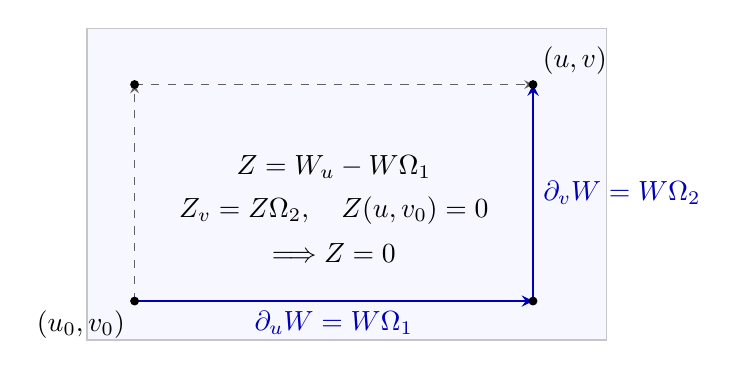
\begin{tikzpicture}[x=1.1cm,y=1.1cm,>=stealth]
	\fill[blue!3] (-0.55,-0.45) rectangle (5.45,3.15);
	\draw[gray!45] (-0.55,-0.45) rectangle (5.45,3.15);
	\draw[->,thick,blue!70!black] (0,0)--node[below] {\(\partial_uW=W\Omega_1\)} (4.6,0);
	\draw[->,thick,blue!70!black] (4.6,0)--node[right] {\(\partial_vW=W\Omega_2\)} (4.6,2.5);
	\draw[->,dashed,gray!75!black] (0,0)--(0,2.5);
	\draw[->,dashed,gray!75!black] (0,2.5)--(4.6,2.5);
	\fill (0,0) circle (1.6pt) node[below left] {\((u_0,v_0)\)};
	\fill (4.6,0) circle (1.6pt);
	\fill (0,2.5) circle (1.6pt);
	\fill (4.6,2.5) circle (1.6pt) node[above right] {\((u,v)\)};
	\node at (2.3,1.55) {\(Z=W_u-W\Omega_1\)};
	\node at (2.3,1.05) {\(Z_v=Z\Omega_2,\quad Z(u,v_0)=0\)};
	\node at (2.3,0.55) {\(\Longrightarrow Z=0\)};
\end{tikzpicture}

	\caption[矩形上的标架积分]{先沿水平线积分，再沿竖线积分。平坦性使横向误差 \(Z\) 始终为零，故交换这两个积分方向也得到同一终点标架。}
	\label{g1:fig:surface-rectangle-integration}
\end{figure}

\subsection{从标架到闭的向量值一形式}
\label{g1:subsec:0804:04}

现在假定给定数据满足 Gauss–Codazzi 条件，在任意包含基点 \(q_0=(u_0,v_0)\) 的矩形 \(V\subseteq U\) 上，用\cref{g1:lem:rectangular-matrix-system}解出初值 \(W_0\in \operatorname{SO}(3)\) 的正交标架 \(W\)，再令
\[
	\mathcal F=WP=(a_1,a_2,n).
\]
由\eqref{g1:eq:surface-orthonormal-frame-system}的定义，
\[
	\partial_i\mathcal F
	=W\Omega_iP+W\partial_iP
	=WPA_i=\mathcal F A_i.
\]
所以 \(a_1,a_2\) 已有了候选切向量应有的导数关系。还欠位置函数 \(X\)：必须证明这两个向量确实能同时写成 \(X_u,X_v\)。

\ProseParagraphBreak

把候选微分写作
\[
	\alpha=a_1\,\mathrm{d}u+a_2\,\mathrm{d}v.
\]
这是一个\term[xiangliangzhiyixingshi]{向量值一形式}[vector-valued 1-form]；这里，它将参数平面中的位移 \((\xi^1,\xi^2)\) 送到向量 \(a_1\xi^1+a_2\xi^2\)。若它的每个实分量都满足混合偏导条件，就称它为闭的；该条件写作
\[
	\mathrm{d}\alpha=(\partial_u a_2-\partial_v a_1)\,\mathrm{d}u\wedge \mathrm{d}v=0.
\]
这里 \(\mathrm{d}u\wedge \mathrm{d}v\) 只记录两个方向交换时变号；不需要预先掌握微分形式的一般理论。由 \(\partial_i\mathcal F=\mathcal F A_i\) 的前两列，
\[
	\partial_u a_2-\partial_v a_1
	=(\Gamma^1_{12}-\Gamma^1_{21})a_1
	+(\Gamma^2_{12}-\Gamma^2_{21})a_2+(h_{12}-h_{21})n=0.
\]
这一步说明了两种对称性的不同职责：Gauss–Codazzi 条件先使标架能够积分，而 \(\Gamma^k_{12}=\Gamma^k_{21}\)、\(h_{12}=h_{21}\) 再使位置的候选微分闭合。两步缺一不可。

\subsection{浸入的构造和秩检验}
\label{g1:subsec:0804:05}

在矩形上，把闭的向量值一形式积分成位置无需调用另一个一般存在定理。指定 \(x_0\in\mathbb R^3\)，直接沿刚才的折线定义
\begin{equation}
	\label{g1:eq:surface-position-rectangle-integral}
	X(u,v)=x_0+\int_{u_0}^u a_1(s,v_0)\,\mathrm{d}s+\int_{v_0}^v a_2(u,t)\,\mathrm{d}t.
\end{equation}
对 \(v\) 求导得到 \(X_v=a_2\)。对 \(u\) 求导，并用 \(\partial_u a_2=\partial_v a_1\)，得到
\[
	X_u=a_1(u,v_0)+\int_{v_0}^v\partial_u a_2(u,t)\,\mathrm{d}t
	=a_1(u,v_0)+a_1(u,v)-a_1(u,v_0)=a_1(u,v).
\]
于是 \(\mathrm{d}X=\alpha\)，且 \(X(q_0)=x_0\)。积分中各函数光滑，故 \(X\) 光滑。

\ProseParagraphBreak

有了位置函数还不能直接宣布它是正则曲面，必须检查两个切向量处处独立。由 \(W^{\mathsf T}W=I\) 及 \(P^{\mathsf T}P=\mathcal G\)，对任意 \(\xi=(\xi^1,\xi^2)\in\mathbb R^2\)，
\[
	\|\mathrm{d}X(\xi)\|^2
	=\|a_1\xi^1+a_2\xi^2\|^2
	=g_{ij}\xi^i\xi^j.
\]
当 \(\xi\ne0\) 时，正定性使右端严格为正，因此 \(\mathrm{d}X\) 的核为零、秩为 \(2\)。这正是最初坚持 \(g\) 正定的原因；若它退化，即使所有偏导相容，也不能保证得到浸入。

\subsection{两基本形式的恢复}
\label{g1:subsec:0804:06}

构造出了浸入，还须核对它实现的是原先的数据。第一基本形式由 \(\mathcal F^{\mathsf T}\mathcal F=\mathcal G\) 立即得到：
\[
	\langle X_i,X_j\rangle=\langle a_i,a_j\rangle=g_{ij}.
\]
从\eqref{g1:eq:surface-metric-factor}的列向量关系得到
\[
	X_u\times X_v=a_1\times a_2=\sqrt D\,n,
\]
故标架第三列确实等于按参数顺序选择的单位法向 \((X_u\times X_v)/\|X_u\times X_v\|\)。取 \(\partial_i\mathcal F=\mathcal F A_i\) 的第 \(j\) 列，
\[
	X_{ij}=\Gamma^1_{ij}X_u+\Gamma^2_{ij}X_v+h_{ij}n.
\]
与 \(n\) 作内积即得 \(\langle X_{ij},n\rangle=h_{ij}\)，所以第二基本形式也恢复了。特别地，第二基本形式的符号并非由事后任取法向决定；构造中的 \(P\) 和 \(W\in \operatorname{SO}(3)\) 已使它与给定参数方向一致。

\begin{example}[平直度量配上非零弯曲]
	\label{g1:exm:fundamental-cylinder-data}
	取 \(g=\mathrm{d}u^2+\mathrm{d}v^2\)、\(h=\lambda\,\mathrm{d}u^2\)，其中 \(\lambda\ne0\) 为常数。此时 \(\Gamma=0\)、\(K_g=0\)、\(\det h=0\)，Codazzi 条件也因系数常数而成立。取 \(P=I\)、\(W(0,0)=I\)，系统成为
	\[
		A_1=\begin{pmatrix}0&0&-\lambda\\0&0&0\\\lambda&0&0\end{pmatrix},
		\qquad A_2=0.
	\]
	于是
	\[
		a_1=(\cos\lambda u,0,\sin\lambda u),\quad
		a_2=(0,1,0),\quad n=(-\sin\lambda u,0,\cos\lambda u).
	\]
	以 \(X(0,0)=0\) 积分，得到
	\[
		X(u,v)=\left(\frac{\sin\lambda u}{\lambda},\,v,\,
		\frac{1-\cos\lambda u}{\lambda}\right).
	\]
	这是半径 \(1/|\lambda|\) 的圆柱面参数化。平直的长度数据允许一个切向方向发生弯曲；Gauss 方程只要求两个主曲率的乘积为零，并不要求每个主曲率都为零。
\end{example}

\subsection{局部唯一性与整体单值}
\label{g1:subsec:0804:07}

现在把构造和唯一性合并成完整结论。初始标架所规定的是两个切向量按顺序正交归一化后的方向，而不是任意指定 \(X_u,X_v\) 的长度；后者已由 \(g\) 给定。

\begin{theorem}[曲面基本定理]
	\label{g1:thm:surface-fundamental}
	设 \(U\subseteq\mathbb R^2\) 为开集，\(g=(g_{ij})\) 为光滑正定对称矩阵，\(h=(h_{ij})\) 为光滑对称矩阵，各矩阵均为 \(2\times2\)。令 \((g^{ij})=g^{-1}\)，\(\Gamma\) 为 \(g\) 的 Christoffel 系数，\(\nabla_i\partial_j=\Gamma^k_{ij}\partial_k\)，\(R\) 为该联络的曲率，约定 \(R(V,W)Z=\nabla_V\nabla_WZ-\nabla_W\nabla_VZ-\nabla_{[V,W]}Z\)。以 \(R(\partial_1,\partial_2)\partial_j=R^k{}_{j12}\partial_k\) 定义分量，令 \(h_i{}^k=g^{k\ell}h_{i\ell}\)、\(\nabla_i h_{jk}=\partial_i h_{jk}-\Gamma^\ell_{ij}h_{\ell k}-\Gamma^\ell_{ik}h_{j\ell}\)，要求 \(R^k{}_{j12}=h_1{}^kh_{2j}-h_2{}^kh_{1j}\) 及 \(\nabla_1h_{2j}=\nabla_2h_{1j}\) 对 \(j,k=1,2\) 成立，即\eqref{g1:eq:surface-data-gauss}、\eqref{g1:eq:surface-data-codazzi}。令 \(E=g_{11}\)、\(F=g_{12}\)、\(D=\det g\)，并令 \(P=\begin{psmallmatrix}\sqrt E&F/\sqrt E&0\\0&\sqrt D/\sqrt E&0\\0&0&1\end{psmallmatrix}\)。给定 \(q_0=(u_0,v_0)\in U\)、\(x_0\in\mathbb R^3\) 及右手正交标架矩阵 \(W_0\in\operatorname{SO}(3)\)，则在每个含 \(q_0\) 的开矩形 \(V\subseteq U\) 上，存在唯一的光滑浸入 \(X\colon V\rightarrow\mathbb R^3\)，其第一、第二基本形式分别为 \(g,h\)，且
	\[
		X(q_0)=x_0,\qquad
		(X_u,X_v,n)(q_0)=W_0P(q_0),\qquad
		n=\frac{X_u\times X_v}{\|X_u\times X_v\|}.
	\]
	这里 \(P\) 由\eqref{g1:eq:surface-metric-factor}确定。若不指定这些初值，同一矩形上的任意两个这样的浸入满足
	\[
		\widetilde X=QX+b,\qquad Q\in \operatorname{SO}(3),\quad b\in\mathbb R^3.
	\]
	这一结论称为\term[qumianjibendingli]{曲面基本定理}[fundamental theorem of surface theory]。
\end{theorem}

\begin{proof}
	由\cref{g1:prop:surface-data-flatness}及\eqref{g1:eq:surface-flatness-change-frame}，\(\Omega_1,\Omega_2\) 满足平坦性；它们的斜对称性已由\eqref{g1:eq:surface-matrix-metric-compatibility}证明。\cref{g1:lem:rectangular-matrix-system}给出初值为 \(W_0\) 的 \(\operatorname{SO}(3)\) 值解。于是前面三小节的构造依次给出闭的候选微分、\eqref{g1:eq:surface-position-rectangle-integral}中的光滑浸入，以及其基本形式和法向的逐项核验，这证明存在性。

	对于任意另一个具有相同数据的浸入 \(\widetilde X\)，\cref{g1:prop:gauss-weingarten}使其坐标标架 \(\widetilde{\mathcal F}=(\widetilde X_u,\widetilde X_v,\widetilde n)\) 满足相同的 \(\partial_i\widetilde{\mathcal F}=\widetilde{\mathcal F}A_i\)。因 \(g\) 相同，\(\widetilde W=\widetilde{\mathcal F}P^{-1}\) 满足同一正交标架系统。若初值也相同，矩形积分引理的唯一性给出 \(\widetilde W=W\)，从而 \(\mathrm{d}\widetilde X=\mathrm{d}X\)。两者之差的两个偏导都为零，沿水平、竖直线段积分可知其在矩形上为常数；基点位置相同便使这个常数为零。

	若不指定初值，令 \(Q=\widetilde W(q_0)W(q_0)^{\mathsf T}\in \operatorname{SO}(3)\)。矩阵 \(QW\) 满足与 \(\widetilde W\) 相同的系统和初值，因此 \(\widetilde W=QW\)。于是 \(\mathrm{d}\widetilde X=Q\,\mathrm{d}X\)，积分得到 \(\widetilde X=QX+b\)，其中 \(b=\widetilde X(q_0)-QX(q_0)\)。
\end{proof}

这里的“唯一”保留了参数点之间的对应；若允许重新参数化，就必须同时按该坐标变换拉回 \(g,h\)。此外，保向刚性变换的限定与法向约定有关：若用一个行列式为 \(-1\) 的正交矩阵反射曲面，按参数叉积重新选择的法向会多出一个负号，第二基本形式随之变号。

\ProseParagraphBreak

对一般开集，定理保证每点附近的局部实现。若沿一条道路继续这些局部解，相交处可用同一位置和标架初值保证它们一致；每一段有限道路只需有限多个小矩形。但绕环路回来时，标架可能已经转动，或者标架虽回到原值，位置却发生平移。这与\cref{g1:prop:periodic-curve-closure}中“标架回到初值”和“位移积分为零”两个条件的区别相同。以下两个例子直接显示这两种障碍，而不把局部存在性误当成任意区域上的单值存在性。

\begin{example}[转动障碍与位移障碍]
	\label{g1:exm:surface-monodromy-obstructions}
	在环带 \(A=\{(x,y):1<\sqrt{x^2+y^2}<2\}\) 上，写 \(r=\sqrt{x^2+y^2}\)。角度 \(\theta\) 不是整个环带上的单值实函数，但
	\[
		\mathrm{d}r=\frac{x\,\mathrm{d}x+y\,\mathrm{d}y}{r},\qquad
		\mathrm{d}\theta=\frac{-y\,\mathrm{d}x+x\,\mathrm{d}y}{r^2}
	\]
	都是单值的一形式；局部选定角度后，它们就是通常的坐标微分。

	先取 \(g=\mathrm{d}r^2+c^2r^2\mathrm{d}\theta^2\)、\(h=0\)，其中 \(c>0\)。在展开角度的矩形 \((1,2)\times\mathbb R\) 上，
	\[
		\widetilde X(r,\theta)=(r\cos c\theta,r\sin c\theta,0)
	\]
	实现这两组数据，因而各局部坐标中的 Gauss–Codazzi 条件都成立。它的单位径向、角向标架绕一周后旋转 \(2\pi c\)。若 \(c\notin\mathbb Z\)，这个标架不能在 \(\theta\) 与 \(\theta+2\pi\) 处匹配。假如环带上有实现数据的单值浸入，把它写到展开角度的矩形上，再用曲面基本定理的唯一性，它必与 \(\widetilde X\) 相差固定保向刚性变换；但固定刚性变换不能消除标架的不匹配，故这样的浸入不存在。

	再取 \(g=\mathrm{d}r^2+\mathrm{d}\theta^2\)、\(h=0\)。在展开角度的矩形上，\(\widetilde X(r,\theta)=(r,\theta,0)\) 实现数据，沿径向、角向的标架都是常向量，已经没有转动障碍。然而候选位置微分为 \(\alpha=(\mathrm{d}r,\mathrm{d}\theta,0)\)，沿任一正向圆周积分得到
	\[
		\oint\alpha=(0,2\pi,0)\ne0.
	\]
	一个单值位置函数的微分沿环路积分必须等于终点减起点，即零；这里却存在非零位移。也可直接由 \(\widetilde X(r,\theta+2\pi)-\widetilde X(r,\theta)=(0,2\pi,0)\) 和同样的唯一性论证排除整体浸入。
\end{example}

这两个例子中的数据处处光滑并且满足相容方程，障碍只在绕环带一周后出现。因而 Gauss–Codazzi 方程精确回答了局部能否实现的问题；在带孔区域上还要另查标架运输和环路位移，不能仅检查点上的曲率等式。

% !TeX root = ../../Book1.tex
% 纲要标题：### 8.5 模型、形变与刚性的界线
% 纲要位置：几何学计划纲要.md，第 453 行。
% 正文状态：初稿；尚未正式审核。

% 纲要内容开始
% 
% * 球面、圆柱和旋转曲面的核验
% * 平面与圆柱的局部等距
% * 一阶、局部和整体刚性问题的区分
% 
% ---
% 
% 纲要内容结束

\section{模型、形变与刚性的界线}
\label{g1:sec:0805}

曲面基本定理需要同时给定 \(I\) 和 \(II\)。如果只给 \(I\)，内在曲率虽然已经确定，两个主曲率及曲面在空间中的形状却还可能变化。本节把这种自由算在几个熟悉模型上，再区分三个常被混在一起的问题：一个变动在一阶上是否保持度量，是否存在真实的等距形变，以及局部构造能否在整张曲面上成立。

\subsection{球面、圆柱和旋转曲面的核验}
\label{g1:subsec:0805:01}

\begin{example}[球面与法向的符号]\label{g1:exm:sphere-two-forms}
	半径 \(R>0\) 的球面去掉两极后，可在经度的局部区间中用
	\[
		X(s,\theta)=\bigl(R\sin(s/R)\cos\theta,\ R\sin(s/R)\sin\theta,\ R\cos(s/R)\bigr),
		\quad 0<s<\pi R
	\]
	参数化。直接求导得到
	\[
		I=\mathrm{d}s^2+R^2\sin^2(s/R)\,\mathrm{d}\theta^2,\qquad
		n=\frac{X}{R}=\frac{X_s\times X_\theta}{\|X_s\times X_\theta\|}.
	\]
	因为 \(\mathrm{d}n=\mathrm{d}X/R\)，本书约定 \(S=-\mathrm{d}n\) 给出 \(S=-R^{-1}\operatorname{id}\)，所以
	\[
		II=-R^{-1}I,\qquad k_1=k_2=-R^{-1},\qquad H=-R^{-1},\qquad K=R^{-2}.
	\]
	因此标准球面仍有正的 Gauss 曲率；外向法向下主曲率为负，与 \(S=-\mathrm{d}n\) 一致。反向选择法向时 \(II,H,k_1,k_2\) 改号，\(I,K\) 不变。参数在两极退化，因为 \(X_\theta=0\)，但球面本身在那里可以改用图像坐标，没有几何奇点。
\end{example}

\begin{example}[圆柱的两个方向]\label{g1:exm:cylinder-two-forms}
	取
	\[
		C(u,v)=\bigl(R\cos(u/R),R\sin(u/R),v\bigr),\qquad R>0.
	\]
	有 \(C_u=(-\sin(u/R),\cos(u/R),0)\)、\(C_v=(0,0,1)\)，两者单位且正交。外向法向 \(n=(\cos(u/R),\sin(u/R),0)\) 等于 \(C_u\times C_v\)，而
	\[
		n_u=R^{-1}C_u,\qquad n_v=0.
	\]
	故
	\[
		I=\mathrm{d}u^2+\mathrm{d}v^2,\qquad II=-R^{-1}\mathrm{d}u^2,\qquad
		k_1=-R^{-1},\quad k_2=0,\quad H=-\frac1{2R},\quad K=0.
	\]
	圆周方向发生弯曲，母线方向没有法向弯曲。这里有一个零主曲率并不表示整张曲面是平面，也不表示参数不正则。
\end{example}

这两例都可由旋转曲面的统一公式找回。取光滑单位速率平面曲线 \((r(s),z(s))\)，假设 \(r>0\) 且 \(r'^2+z'^2=1\)，绕 \(z\) 轴旋转：
\[
	X(s,\theta)=(r(s)\cos\theta,r(s)\sin\theta,z(s)).
\]
弧长条件只作用于母线；\(\theta\) 方向的长度因子仍为 \(r\)。

\begin{proposition}[旋转曲面的基本形式]\label{g1:prop:revolution-two-forms}
	在上述光滑单位速率母线、\(r>0\) 及局部角参数条件下，选择法向
	\[
		n=(-z'\cos\theta,-z'\sin\theta,r'),
	\]
	则
	\[
		I=\mathrm{d}s^2+r^2\mathrm{d}\theta^2,\qquad
		II=(r'z''-z'r'')\,\mathrm{d}s^2+rz'\,\mathrm{d}\theta^2.
	\]
	子午线和纬线方向为主方向，主曲率及 Gauss 曲率为
	\begin{equation}\label{g1:eq:revolution-curvatures}
		k_s=r'z''-z'r'',\qquad k_\theta=\frac{z'}r,\qquad
		K=-\frac{r''}r,\qquad H=\frac12\left(r'z''-z'r''+\frac{z'}r\right).
	\end{equation}
	在脐点，这两方向仍是主方向，但不再是仅有的主方向。
\end{proposition}

\begin{proof}
	计算 \(X_s,X_\theta\) 得到 \(\|X_s\|=1\)、\(\|X_\theta\|=r\)、\(\langle X_s,X_\theta\rangle=0\)，且 \(X_s\times X_\theta=rn\)。二阶导数与 \(n\) 的内积分别是
	\[
		\langle X_{ss},n\rangle=-z'r''+r'z'',\qquad
		\langle X_{s\theta},n\rangle=0,\qquad
		\langle X_{\theta\theta},n\rangle=rz'.
	\]
	因此 \(I,II\) 都对角，形算子的两个特征值是相应对角项之比。最后，由单位速率条件求导得 \(r'r''+z'z''=0\)，从而
	\[
		z'(r'z''-z'r'')=-r'^2r''-z'^2r''=-r'',
	\]
	即得 \(K=-r''/r\)。此推导没有除以 \(z'\)，故 \(z'=0\) 的点也包括在内。
\end{proof}

令 \(r=R\sin(s/R),z=R\cos(s/R)\)，就得到外向球面的两个负主曲率。令 \(r=R,z=s\)，则上面指定的法向朝向圆柱轴线，因而 \(k_\theta=1/R\)；它与前一例的负号差别完全来自法向，不能直接混用。对圆锥的去顶点部分，取 \(r=as,z=bs\)，其中 \(s>0,a>0,a^2+b^2=1\)，可得 \(K=0\)。\(r=0\) 的顶点不属于命题的适用区域，零曲率公式不能被延伸为顶点正则性的证明。

\begin{example}[一个非平面的负曲率模型]\label{g1:exm:catenoid-curvatures}
	取 \(r(s)=\sqrt{a^2+s^2}\)、\(z(s)=a\,\operatorname{arsinh}(s/a)\)，其中 \(a>0\)。这里 \(\operatorname{arsinh}\) 是双曲正弦的反函数，导数为 \(1/\sqrt{1+t^2}\)。计算得
	\[
		r'=\frac{s}{r},\quad z'=\frac ar,\quad
		r''=\frac{a^2}{r^3},\quad z''=-\frac{as}{r^3}.
	\]
	因此母线确实单位速率，而旋转曲面的 \(k_s=-a/r^2\)、\(k_\theta=a/r^2\)，故 \(H=0\)、\(K=-a^2/r^4<0\)。这是\term[xuanlianmian]{悬链面}[catenoid]的一个弧长参数表示。平均曲率为零表示两个带符号主曲率相互抵消，绝不是两个主曲率都为零。
\end{example}

\subsection{平面与圆柱的局部等距}
\label{g1:subsec:0805:02}

平面 \(P(u,v)=(u,v,0)\) 与圆柱参数 \(C(u,v)\) 的第一基本形式都为 \(\mathrm{d}u^2+\mathrm{d}v^2\)。在宽度小于 \(2\pi R\) 的开条带上，\(C\) 单射，故对应 \(P(u,v)\mapsto C(u,v)\) 是局部曲面之间的等距。由\cref{g1:prop:local-isometry-length}，任意纸上曲线的长度以及相交角度都保持；这正是“无拉伸卷起”的数学含义。

\ProseParagraphBreak

它不可能由空间刚性运动得到：平面的第二基本形式恒为零，而圆柱的第二基本形式不为零；刚性运动保持第二基本形式（同时推送所选法向），反射至多因法向约定带来整体改号，也不能把零变成非零。第一基本形式的相同因此不足以触发上一节的曲面唯一性结论。

\begin{example}[从平面连续卷起]\label{g1:exm:plane-cylinder-bending}
	在固定有界矩形 \(U=(-a,a)\times(-b,b)\) 上定义
	\[
		X_t(u,v)=
		\begin{cases}
			\bigl(\sin(tu)/t,\ v,\ (1-\cos(tu))/t\bigr),&t\ne0,\\
			(u,v,0),&t=0.
		\end{cases}
	\]
	函数 \(\sin(tu)/t=\int_0^u\cos(t\xi)\,\mathrm{d}\xi\)、\((1-\cos(tu))/t=\int_0^u\sin(t\xi)\,\mathrm{d}\xi\) 表明 \(X_t\) 对 \((t,u,v)\) 光滑，并无真实的 \(t=0\) 奇点。因为
	\[
		(X_t)_u=(\cos(tu),0,\sin(tu)),\qquad (X_t)_v=(0,1,0),
	\]
	全部 \(t\) 对应的第一基本形式都为 \(\mathrm{d}u^2+\mathrm{d}v^2\)。取 \(n_t=(-\sin(tu),0,\cos(tu))\)，则 \(II_t=t\,\mathrm{d}u^2\)。当 \(|t|a<\pi/2\) 时第一坐标对 \(u\) 严格递增，故每个 \(X_t\) 还是嵌入。这个例子既给出真实的局部等距形变，又清楚显示被改变的数据是第二基本形式。
\end{example}

\cref{g1:fig:plane-cylinder-bending}画出同一参数网格在 \(t=0\) 与 \(t=1\) 时的样子。网格线在图纸上的投影长度可以不同；被保持的是曲面自身的 \(I\)，并非观看图像时的平面投影距离。

% !TeX root = ../Book1.tex
\begin{figure}[htbp]
	\centering
	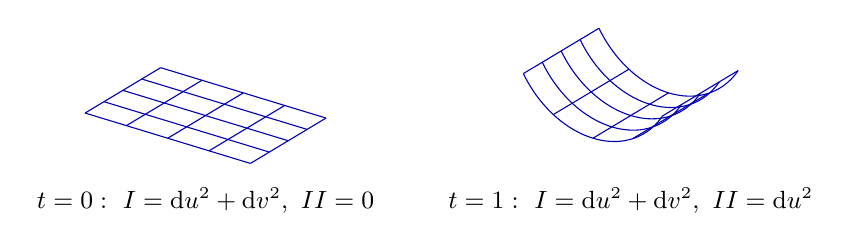
\begin{tikzpicture}[x={(1.05cm,-0.32cm)},y={(0.6cm,0.36cm)},z={(0cm,1.2cm)},font=\small]
		\begin{scope}[xshift=-2.8cm]
			\foreach \a in {-1,-0.5,0,0.5,1}{\draw[blue!70!black] (\a,-0.8,0)--(\a,0.8,0);}
			\foreach \b in {-0.8,-0.4,0,0.4,0.8}{\draw[blue!70!black] (-1,\b,0)--(1,\b,0);}
			\node at (0,0,-0.9) {\(t=0:\ I=\mathrm{d}u^2+\mathrm{d}v^2,\ II=0\)};
		\end{scope}
		\begin{scope}[xshift=2.6cm]
			\foreach \a in {-1,-0.5,0,0.5,1}{\draw[blue!70!black] ({sin(deg(\a))},-0.8,{1-cos(deg(\a))})--({sin(deg(\a))},0.8,{1-cos(deg(\a))});}
			\foreach \b in {-0.8,-0.4,0,0.4,0.8}{\draw[blue!70!black,domain=-1:1,samples=41,variable=\a] plot ({sin(deg(\a))},\b,{1-cos(deg(\a))});}
			\node at (0,0,-0.9) {\(t=1:\ I=\mathrm{d}u^2+\mathrm{d}v^2,\ II=\mathrm{d}u^2\)};
		\end{scope}
	\end{tikzpicture}
	\caption[平面卷成圆柱片]{同一参数网格的等距形变。两图的第一基本形式相同；弯曲后沿 \(u\) 方向的法向随位置改变，第二基本形式随之改变。图中采用例中的法向约定。}
	\label{g1:fig:plane-cylinder-bending}
\end{figure}


如果在整个参数平面上使用 \(C\)，则 \(C(u+2\pi R,v)=C(u,v)\)。它仍逐点保持度量，却不再单射，因而不是平面到整张圆柱的等距。更强地，平面与整张圆柱之间不存在任何整体微分同胚：平面可收缩，而圆柱投影到圆周的映射与固定高度的圆周包含互为收缩关系，绕轴一周的道路不可能收缩成点。后一断言可直接由\cref{g1:thm:circle-fundamental}中 \(\pi_1(S^1)\cong\mathbb Z\) 及投影、包含的复合为恒等得到。这个拓扑障碍与局部度量计算并不矛盾。

\subsection{一阶、局部和整体刚性问题的区分}
\label{g1:subsec:0805:03}

“刚性”必须说明保持什么、在哪个区域比较以及是否允许改变参数。曲面基本定理的唯一性固定了参数域上的两种形式：若两个浸入的 \(I,II\) 相同，才比较它们是否由一个固定的空间刚性运动联系。若给定一个参数对应 \(\phi\)，应先将第二个浸入换成 \(\widetilde X\circ\phi\)，再逐项比较两种形式。

\begin{definition}[无穷小等距变动]\label{g1:def:infinitesimal-bending}
	设 \(X:U\rightarrow\mathbb R^3\) 为光滑浸入，\(V:U\rightarrow\mathbb R^3\) 为沿 \(X\) 的光滑向量场。若
	\begin{equation}\label{g1:eq:infinitesimal-bending}
		\langle\partial_iV,X_j\rangle+\langle X_i,\partial_jV\rangle=0,\qquad i,j=1,2,
	\end{equation}
	称 \(V\) 为一个\term[wuqiongxiaodengjubiandong]{无穷小等距变动}[infinitesimal bending]。若 \(V=a+\Omega X\)，其中 \(a\in\mathbb R^3\) 固定、\(\Omega\) 为固定斜对称矩阵，称其为刚性运动产生的变动。
\end{definition}

几何上 \(V(q)\) 是曲面点最初的移动速度。若光滑族 \(X_t\) 满足 \(X_0=X\)，则对 \(g_{ij}(t)=\langle(X_t)_i,(X_t)_j\rangle\) 求 \(t\) 导数，正好得到\eqref{g1:eq:infinitesimal-bending}，其中 \(V=\partial_tX_t|_{t=0}\)。因此真正的等距形变一定产生无穷小等距变动。斜对称矩阵给出
\[
	\langle\Omega X_i,X_j\rangle+\langle X_i,\Omega X_j\rangle=0,
\]
所以刚性运动产生的变动总满足这个线性方程。

\begin{example}[一阶条件并不足够]\label{g1:exm:nonintegrable-plane-bending}
	对平面 \(X(u,v)=(u,v,0)\)，任意光滑函数 \(f\) 都给出 \(V=f(u,v)(0,0,1)\)，并满足\eqref{g1:eq:infinitesimal-bending}，因为 \(\partial_iV\) 总与平面垂直。它不一定来自真正的等距形变。取 \(f=u^2+v^2\)，假设有对 \((t,u,v)\) 光滑的浸入族 \(X_t\)，使 \(X_0=X\)、\(\partial_tX_t|_0=V\)，且 \(I_t=\mathrm{d}u^2+\mathrm{d}v^2\)。取由参数定向决定的法向 \(n_t\)。因为 \(X_{ij}|_{t=0}=0\)，
	\[
		h_{ij}(0)=0,\qquad
		\left.\partial_t h_{ij}(t)\right|_0
		=\langle\partial_i\partial_jV,(0,0,1)\rangle=f_{ij}.
	\]
	因此在任一固定参数点有 \(h(t)=2tI_2+O(t^2)\)，从而 \(\det h(t)=4t^2+O(t^3)\)。可是固定的平面度量具有 \(K=0\)，由\cref{g1:thm:gauss-equation}必须有 \(\det h(t)=K\det g=0\)，矛盾。这里一阶约束全满足，二阶相容性却阻止了真实形变。
\end{example}

相比之下，\cref{g1:exm:plane-cylinder-bending}在 \(t=0\) 的变动为 \(V=(u^2/2)(0,0,1)\)，它确实来自整个等距族；其二阶导数矩阵的行列式为零。这个比较只说明上述必要障碍在后一例中消失，不能反过来把“行列式为零”未经证明地宣布为任意形变都可积分的充分条件。

\begin{proposition}[两种形式相同的整体唯一性]\label{g1:prop:surface-global-uniqueness}
	设 \(U\subseteq\mathbb R^2\) 为连通开集，\(X,\widetilde X:U\rightarrow\mathbb R^3\) 为光滑浸入，均取参数定向的单位法向。若两者在同一参数下具有相同的第一、第二基本形式，则存在一个固定 \(Q\in \operatorname{SO}(3)\) 和 \(a\in\mathbb R^3\)，使 \(\widetilde X=QX+a\) 在整个 \(U\) 上成立。这里不要求 \(U\) 单连通。
\end{proposition}

\begin{proof}
	在一点由两组标架与位置确定 \(Q,a\)，再将 \(\widetilde X\) 替换为 \(Q^{-1}(\widetilde X-a)\)。设两者的位置、两个一阶偏导及法向全部相同的点集为 \(A\)。这个集合非空，由连续性为闭集。每个 \(q\in A\) 都有一个矩形邻域；\cref{g1:thm:surface-fundamental}中指定位置及标架初值的唯一性使两浸入在该矩形内相同，所以 \(A\) 也开。连通性给出 \(A=U\)。只比较已经存在的两个整体解时，不会发生“沿不同道路构造出不同解”的问题，因此无需用单连通性排除运输障碍。
\end{proof}

由此可见，局部存在、整体存在与整体唯一性有不同的条件。相容性给出小邻域上的实现；绕闭路运输能否回到同一标架和同一位置，决定能否将局部实现接成单值的整体实现；两个已经存在的实现若保持全部数据，其唯一性又可由连通性传播。本章没有把仅保持第一基本形式的闭曲面刚性问题归结为这一命题。


\begin{chaptersummary}
	浸入要求两个参数方向在空间中仍然独立，它只保证局部图像模型。第一基本形式是切向量的内积，按坐标换元公式转换；长度、面积、梯度、散度与 Laplace 算子由它确定。参数矩阵的样子可以改变，而内积及其测量含义不改变。局部等距保持这套数据，却可能改变曲面在空间中的形状。

	\ProseParagraphBreak

	固定法向以后，形算子 \(S=-\mathrm{d}n\) 和第二基本形式记录法向弯曲。自伴性给出正交主方向，Euler 公式把任意方向的法曲率写成两个主曲率的加权平均。平均曲率与 Gauss 曲率分别是半迹与行列式；法向反转使前者改号，却不改变后者。脐点、零主曲率和渐近方向的退化须逐项区分，不能从一个点的二阶数据直接推出邻域的形状。

	\ProseParagraphBreak

	结构方程把坐标标架的导数分为切向与法向两部分。协变导数记录切向变化，其系数由度量决定；混合偏导相容性同时给出 Gauss 与 Codazzi 方程。Gauss 方程使两个主曲率的乘积成为内在量，这解释了球面不能局部等距铺平，也解释了平面和圆柱虽有相同的零 Gauss 曲率，仍可有不同的主曲率。

	\ProseParagraphBreak

	反向构造先把给定度量分解为标架的长度约束，再把相容条件转为矩阵系统的平坦性。两次普通微分方程积分、误差的零初值唯一性，以及闭向量值一形式的显式积分，共同得到局部浸入；正定性落实秩为二，列向量的内积和导数恢复全部数据。在同一参数下，两种形式共同决定曲面到保向刚性运动为止。整体单值还可能遇到转动或位移障碍，整体单射和仅保持度量的刚性则是进一步的问题。
\end{chaptersummary}

\BookExercises
以下习题均附完整解答。计算前先固定参数和法向；使用存在或唯一性结论时，区分给定的是第一基本形式、两种基本形式，还是只有它们的一阶变化。

\begin{exercise}\label{g1:ex:oblique-metric-measurements}
	对 \(X(u,v)=(u+v,v,0)\)，求参数单位正方形的面积、两条对角线的长度及函数 \(f(u,v)=u\) 的曲面梯度。说明参数分量 \((1,0)\) 为什么不是该梯度。
\end{exercise}
\begin{solution}
	度量矩阵及其逆为
	\[
		g=\begin{pmatrix}1&1\\1&2\end{pmatrix},\qquad
		g^{-1}=\begin{pmatrix}2&-1\\-1&1\end{pmatrix},\qquad D=1.
	\]
	故单位正方形的像为面积 \(1\) 的平行四边形。两条对角线的参数方向分别是 \((1,1)\) 与 \((1,-1)\)，在参数长度为 \(1\) 的区间上走过，平方速度分别为 \(5\) 与 \(1\)，所以长度为 \(\sqrt5\) 与 \(1\)。

	由\eqref{g1:eq:surface-gradient}，\(\operatorname{grad}_gf=2\partial_u-\partial_v\)，空间向量为 \(2X_u-X_v=(1,-1,0)\)。空间平面上 \(f=x-y\)，确实有这个 Euclid 梯度。如果误用 \(\partial_u\)，则它与 \(\partial_v\) 的内积是 \(g_{12}=1\)，而 \(\mathrm{d}f(\partial_v)=0\)，不满足梯度的定义。
\end{solution}

\begin{exercise}\label{g1:ex:graph-area-gradient}
	设 \(X(u,v)=(u,v,f(u,v))\) 为光滑图像，令 \(w=(f_u,f_v)^{\mathsf T}\)。
	\begin{enumerate}
		\item 证明 \(g=I_2+ww^{\mathsf T}\)，并求 \(D\)、\(g^{-1}\) 与高度函数 \(f\) 的曲面梯度。
		\item 对 \(f=(u^2+v^2)/2\)，求参数圆盘 \(u^2+v^2\le R^2\) 对应曲面片的面积。
	\end{enumerate}
\end{exercise}
\begin{solution}
	1. 由 \(X_u=(1,0,f_u),X_v=(0,1,f_v)\)，立即得到所给矩阵。展开二阶行列式，有 \(D=1+|w|^2\)。直接相乘可验
	\[
		(I_2+ww^{\mathsf T})\left(I_2-\frac{ww^{\mathsf T}}{1+|w|^2}\right)=I_2,
	\]
	所以 \(g^{-1}=I_2-ww^{\mathsf T}/(1+|w|^2)\)。于是梯度的参数分量为 \(w/(1+|w|^2)\)，对应空间向量
	\[
		\operatorname{grad}f=\frac{(f_u,f_v,f_u^2+f_v^2)}{1+f_u^2+f_v^2}.
	\]
	它也等于 \((0,0,1)-\langle(0,0,1),n\rangle n\)，其中 \(n=(-f_u,-f_v,1)/\sqrt{1+|w|^2}\)，与投影解释相符。

	2. 此时 \(D=1+u^2+v^2\)，用平面极坐标积分得
	\[
		\operatorname{Area}=2\pi\int_0^Rr\sqrt{1+r^2}\,\mathrm{d}r
		=\frac{2\pi}{3}\bigl((1+R^2)^{3/2}-1\bigr).
	\]
	被积函数中的一个 \(r\) 来自参数平面的极坐标换元，\(\sqrt{1+r^2}\) 才是图像的面积伸缩因子；两者不可遗漏或混同。
\end{solution}

\begin{exercise}\label{g1:ex:conformal-laplacian}
	在平面开集 \(U\) 上取 \(g=e^{2\phi}(\mathrm{d}u^2+\mathrm{d}v^2)\)，其中 \(\phi\) 光滑。求 \(\operatorname{grad}_gf\) 和 \(\Delta_gf\)，并证明对任意 \(f\in C_c^\infty(U)\)，积分 \(\int_U|\operatorname{grad}_gf|_g^2\,\mathrm{d}A_g\) 与 \(\phi\) 无关。由此判断，在这个度量下满足 \(\Delta_gf=0\) 的函数是否与 Euclid 度量下相同。
\end{exercise}
\begin{solution}
	这里 \(g^{ij}=e^{-2\phi}\delta_{ij}\)，\(\sqrt D=e^{2\phi}\)。因此
	\[
		\operatorname{grad}_gf=e^{-2\phi}(f_u\partial_u+f_v\partial_v),\qquad
		\Delta_gf=-e^{-2\phi}(f_{uu}+f_{vv}).
	\]
	散度中的乘积 \(\sqrt D\,g^{ij}\) 恰为 \(\delta_{ij}\)，这就是没有出现 \(\phi\) 的导数的原因。又
	\[
		|\operatorname{grad}_gf|_g^2=e^{-2\phi}(f_u^2+f_v^2),
		\qquad
		\int_U|\operatorname{grad}_gf|_g^2\,\mathrm{d}A_g
		=\int_U(f_u^2+f_v^2)\,\mathrm{d}u\,\mathrm{d}v.
	\]
	因 \(e^{-2\phi}>0\)，\(\Delta_gf=0\) 等价于 \(f_{uu}+f_{vv}=0\)，解的集合确实相同；不过算子本身和度量长度通常不同，不能因此把两个度量判为等距。
\end{solution}

\begin{exercise}\label{g1:ex:area-angle-not-isometry}
	在两个标准 Euclid 平面之间，分别考虑 \(\phi(u,v)=(2u,v/2)\) 和 \(\psi(u,v)=(2u,2v)\)。判断它们是否保持面积、是否保持夹角、是否局部等距，并为每个否定结论给出具体的方向或区域。
\end{exercise}
\begin{solution}
	\(\phi\) 的导数行列式为 \(1\)，故由面积换元保持每个区域的面积。但 \((1,0)\) 的长度从 \(1\) 变为 \(2\)，所以不是局部等距。原来正交的方向 \(a=(1,1)\)、\(b=(1,-1)\) 映为 \((2,1/2)\)、\((2,-1/2)\)，内积为 \(15/4\ne0\)，故也不保持夹角。

	\(\psi\) 把内积乘以 \(4\)，向量长度乘以 \(2\)，夹角公式中的因子抵消，故保持夹角；但单位正方形面积变成 \(4\)，单位线段长度变成 \(2\)，所以既不保持面积，也不是局部等距。单独保持面积或单独保持夹角都不足以代替第一基本形式的完整条件。
\end{solution}

\begin{exercise}\label{g1:ex:shape-oblique-basis}
	在某曲面的一点，以坐标切基 \(X_1,X_2\) 表示的两基本形式矩阵为
	\[
		g=\begin{pmatrix}2&1\\1&1\end{pmatrix},\qquad h=\begin{pmatrix}2&0\\0&-1\end{pmatrix}.
	\]
	求形算子矩阵、主曲率及一组正交单位主向量，并求沿 \(X_1,X_2\) 的法曲率。形算子矩阵不是通常的对称矩阵，为什么不违反其自伴性？
\end{exercise}
\begin{solution}
	因为 \(\det g=1\)，
	\[
		[S]=g^{-1}h=\begin{pmatrix}1&-1\\-1&2\end{pmatrix}
		\begin{pmatrix}2&0\\0&-1\end{pmatrix}
		=\begin{pmatrix}2&1\\-2&-2\end{pmatrix}.
	\]
	迹为 \(0\)，行列式为 \(-2\)，所以主曲率为 \(k_\pm=\pm\sqrt2\)。对应的特征向量可取
	\[
		w_\pm=X_1+(k_\pm-2)X_2.
	\]
	用给定的 \(g\) 而不是把系数当作直角坐标计算，得到
	\[
		\langle w_+,w_-\rangle
		=2+(k_+-2)+(k_--2)+(k_+-2)(k_--2)=0,
	\]
	且 \(\lVert w_\pm\rVert^2=2+2(k_\pm-2)+(k_\pm-2)^2=4-2k_\pm>0\)。于是 \(e_\pm=w_\pm/\sqrt{4-2k_\pm}\) 是所求正交单位主向量。

	两个坐标方向的法曲率分别为 \(h_{11}/g_{11}=1\) 和 \(h_{22}/g_{22}=-1\)，均不同于主曲率，说明坐标方向并非主方向。自伴性在这个基下应写成 \([S]^{\mathsf T}g=g[S]\)，两边都等于 \(h\)；只有 \(g=I\) 的正交单位基才把这个条件化成矩阵自身对称。
\end{solution}

\begin{exercise}\label{g1:ex:graph-mean-curvature}
	设 \(X(u,v)=(u,v,f(u,v))\) 为光滑图像，取向上法向。推导
	\[
		H=\frac{(1+f_v^2)f_{uu}-2f_uf_vf_{uv}+(1+f_u^2)f_{vv}}
		{2(1+f_u^2+f_v^2)^{3/2}},
		\qquad
		K=\frac{f_{uu}f_{vv}-f_{uv}^2}{(1+f_u^2+f_v^2)^2}.
	\]
	对 \(f(u,v)=u^2-v^2\) 求 \(H,K\)，说明一个点的 \(H=0\) 既不能直接推出整个邻域的 \(H=0\)，也不能推出曲面在该点附近为平面。
\end{exercise}
\begin{solution}
	由\cref{g1:exm:graph-second-form}，令 \(W=\sqrt{1+f_u^2+f_v^2}\)，则 \(E=1+f_u^2\)、\(F=f_uf_v\)、\(G=1+f_v^2\)、\(D=W^2\)，并有 \(h_{ij}=f_{ij}/W\)。分别代入\eqref{g1:eq:surface-HK-formulas}，分子的第二基本形式贡献一个或两个 \(W^{-1}\)，便得到题设的 \(H,K\) 公式。

	对 \(f=u^2-v^2\)，有 \(f_u=2u\)、\(f_v=-2v\)、\(f_{uu}=2\)、\(f_{vv}=-2\)、\(f_{uv}=0\)。因此
	\[
		H=\frac{4(v^2-u^2)}{(1+4u^2+4v^2)^{3/2}},\qquad
		K=\frac{-4}{(1+4u^2+4v^2)^2}.
	\]
	原点 \(H=0\)，但任意邻域都含 \(v^2\ne u^2\) 的点，故 \(H\) 在该邻域不恒为零；而 \(K<0\) 已说明此曲面不是平面。这些计算分别排除了两个推断，原点的平均曲率为零只表示两个主曲率在该点相互抵消。
\end{solution}

\begin{exercise}\label{g1:ex:helicoid-asymptotic-curves}
	先证明曲面内的任意正则直线段都是渐近线。再设 \(a>0\)，考虑
	\[
		X(u,v)=(u\cos v,u\sin v,av),\qquad u>0,\quad v\in\mathbb R.
	\]
	取 \(X_u\times X_v\) 确定的法向，求两基本形式及 \(H,K\)。证明两族坐标曲线都是渐近线，并说明其中一族不是直线，从而否定上述结论的逆命题。
\end{exercise}
\begin{solution}
	直线段改用弧长后加速度为零，由\cref{g1:prop:surface-normal-acceleration}知 \(\mathrm{II}(\gamma',\gamma')=0\)，所以是渐近线。

	对题设曲面，记 \(W=\sqrt{u^2+a^2}\)。有
	\[
		X_u=(\cos v,\sin v,0),\qquad X_v=(-u\sin v,u\cos v,a),\qquad
		n=\frac{(a\sin v,-a\cos v,u)}W.
	\]
	由 \(E=1,F=0,G=W^2\) 可知浸入处处正则。又
	\[
		X_{uu}=0,\qquad X_{uv}=(-\sin v,\cos v,0),\qquad
		X_{vv}=(-u\cos v,-u\sin v,0),
	\]
	与 \(n\) 作内积得到 \(h_{11}=h_{22}=0\)、\(h_{12}=-a/W\)。所以
	\[
		\mathrm I=(\mathrm du)^2+(u^2+a^2)(\mathrm dv)^2,\qquad
		\mathrm{II}=-\frac{2a}{W}\,\mathrm du\,\mathrm dv,\qquad
		H=0,\quad K=-\frac{a^2}{(u^2+a^2)^2}.
	\]
	因 \(a/W\ne0\)，渐近方向恰由 \(\mathrm du\,\mathrm dv=0\) 给出，故 \(u\) 固定与 \(v\) 固定的两族坐标曲线都是渐近线。固定 \(v\) 得到直线；固定 \(u=u_0>0\) 则得到圆柱螺线 \((u_0\cos v,u_0\sin v,av)\)，其曲率为 \(u_0/(u_0^2+a^2)>0\)，不是直线。这与渐近条件并不矛盾：它的加速度沿曲面的切平面，而不是沿曲面法向。
\end{solution}

\begin{exercise}\label{g1:ex:gauss-map-area-factor}
	设光滑浸入 \(X:U\to\mathbb R^3\) 取单位法向 \(n=(X_1\times X_2)/\sqrt D\)。证明
	\[
		n_1\times n_2=K(X_1\times X_2),\qquad
		\lVert n_1\times n_2\rVert=|K|\sqrt D.
	\]
	解释后一式中 \(|K|\) 的面积意义，并用图像 \(z=x^2\) 说明：\(K\) 恒为零也不能推出 Gauss 映射为常值。
\end{exercise}
\begin{solution}
	以 \(X_1,X_2\) 为基，\(n_i=-S(X_i)\)。二维线性变换对有向平行四边形的面积乘以行列式；在这里直接按两个系数展开叉积，也得到
	\[
		n_1\times n_2=(-S(X_1))\times(-S(X_2))
		=\det(-S)(X_1\times X_2)=K(X_1\times X_2).
	\]
	两边取范数，并用 \(\lVert X_1\times X_2\rVert=\sqrt D\)，即得第二式。曲面原来的面积密度为 \(\sqrt D\)，Gauss 映射在单位球面上扫过的参数面积密度为 \(\lVert n_1\times n_2\rVert\)；两者之比是 \(|K|\)。这个说法是局部的面积变化率，若不同参数点映到同一法向，参数面积积分仍会计入各次覆盖。

	对 \(X(u,v)=(u,v,u^2)\)，有
	\[
		n(u,v)=\frac{(-2u,0,1)}{\sqrt{1+4u^2}},\qquad
		h=\frac1{\sqrt{1+4u^2}}\begin{pmatrix}2&0\\0&0\end{pmatrix}.
	\]
	因 \(\det h=0\)，处处 \(K=0\)，但 \(n\) 随 \(u\) 变化。这里 Gauss 映射的微分秩为 \(1\)，所以它没有扫出二维面积，却仍扫过一条球面曲线。行列式为零只表示面积塌缩，并不表示整个微分为零。
\end{solution}


\begin{exercise}\label{g1:ex:polar-parallel-vector}
	在去掉原点的平面上，令 \(e_r=(\cos\theta,\sin\theta,0)\)、\(e_\theta=(-\sin\theta,\cos\theta,0)\)。沿圆周 \(r=r_0>0\)，写切向量场 \(V(\theta)=a(\theta)e_r+b(\theta)e_\theta\)。利用本章的协变导数求出 \(\nabla_{\mathrm d/\mathrm d\theta}V=0\) 的所有解，并解释为什么分量改变而几何向量可以不变。这里沿参数曲线的协变导数指普通导数向平面切空间的投影。
\end{exercise}
\begin{solution}
	平面切空间恒定，普通导数已经是切向量。由 \(\mathrm de_r/\mathrm d\theta=e_\theta\)、\(\mathrm de_\theta/\mathrm d\theta=-e_r\)，
	\[
		\nabla_{\mathrm d/\mathrm d\theta}V
		=(\dot a-b)e_r+(\dot b+a)e_\theta.
	\]
	所以方程等价于 \(\dot a=b\)、\(\dot b=-a\)，其全部解为
	\[
		a=A\cos\theta+B\sin\theta,\qquad
		b=-A\sin\theta+B\cos\theta,
	\]
	其中 \(A,B\) 为常数。可直接代入验证，而任意初值唯一确定 \(A,B\)，也可由\cref{g1:lem:linear-frame-ode}的唯一性确认没有其他解。代回原式，得到 \(V=(A,B,0)\)，确为固定向量。变化的 \(a,b\) 只是相对于旋转基的分量；如果错误地只令 \(\dot a=\dot b=0\)，通常得到的是随圆周一起转动的向量。
\end{solution}

\begin{exercise}\label{g1:ex:two-conformal-metrics}
	\begin{enumerate}
		\item 在 \(\mathbb R^2\) 上考虑 \(g=e^{2u}(\mathrm du^2+\mathrm dv^2)\)。求它的曲率，并验证 \(X(u,v)=(e^u\cos v,e^u\sin v,0)\) 实现这个度量。这个参数化是否是到其像的整体一一对应？
		\item 在上半平面 \(v>0\) 上考虑 \(g=v^{-2}(\mathrm du^2+\mathrm dv^2)\)。求它的曲率，判断它能否局部等距于某个 Euclid 平面开集。
	\end{enumerate}
\end{exercise}
\begin{solution}
	(1) 此时 \(\phi=u\)，所以\eqref{g1:eq:conformal-gauss-curvature}给出 \(K_g=0\)。直接求导，
	\[
		X_u=e^u(\cos v,\sin v,0),\qquad
		X_v=e^u(-\sin v,\cos v,0),
	\]
	二者正交且长度均为 \(e^u\)，所以 \(X\) 是浸入并诱导所给度量。然而 \(X(u,v+2\pi)=X(u,v)\)，它不是整体一一对应。这是局部度量完全实现而参数仍有整体重复的例子。

	(2) 此时 \(\phi=-\log v\)，有 \(\phi_{uu}=0\)、\(\phi_{vv}=v^{-2}\)，故 \(K_g=-v^2\cdot v^{-2}=-1\)。Euclid 平面开集的曲率为零。若存在局部等距，重参数化后度量一致，由\cref{g1:prop:surface-curvature-two-dim}及曲率的坐标公式，曲率也应一致，矛盾。这里仅在参数域上计算给定度量，不需要先假定它在三维空间中存在整体浸入。
\end{solution}

\begin{exercise}\label{g1:ex:gauss-codazzi-independent}
	在参数域 \(U=\{(u,v):v>0\}\) 上取平坦度量 \(g=\mathrm du^2+\mathrm dv^2\)。
	\begin{enumerate}
		\item 令 \(h=v\,\mathrm du^2\)，证明它满足 Gauss 方程，但不满足 Codazzi 方程。
		\item 令 \(h=\mathrm du^2+\mathrm dv^2\)，证明它满足 Codazzi 方程，但不满足 Gauss 方程。
	\end{enumerate}
	由此判断两组数据能否作为某个曲面片的两基本形式。
\end{exercise}
\begin{solution}
	度量系数恒定，所以全部 \(\Gamma^k_{ij}=0\)，从而 \(R=0\)、\(K_g=0\)，且 \(\nabla_i h_{jk}=\partial_i h_{jk}\)。

	(1) 矩阵 \(h=\operatorname{diag}(v,0)\) 的行列式为零，故 \(K_g=\det(g^{-1}h)=0\)。由\cref{g1:prop:surface-curvature-two-dim}，这就是完整的 Gauss 方程。然而
	\[
		\nabla_1h_{21}=0,\qquad \nabla_2h_{11}=1,
	\]
	不满足 Codazzi 方程。

	(2) 矩阵 \(h=I\) 恒定，所有协变导数均为零，故 Codazzi 方程成立。但 \(\det(g^{-1}h)=1\ne0=K_g\)，Gauss 方程不成立。两组数据分别违反一个必要条件，因此均不能在任何非空开子域上作为光滑曲面片的两基本形式。
\end{solution}

\begin{exercise}\label{g1:ex:totally-umbilic-surface}
	设 \(U\subseteq\mathbb R^2\) 是连通开集，\(X\colon U\rightarrow\mathbb R^3\) 是光滑浸入，取光滑单位法向 \(n\)。假设每一点都是脐点，即 \(S=\lambda I\)，其中 \(\lambda\) 为光滑函数。证明 \(\lambda\) 为常数，并证明 \(X(U)\) 包含在某个平面或某个球面中。说明只在一个点为脐点为什么不足以得到这个结论。
\end{exercise}
\begin{solution}
	由 \(\nabla_V(\lambda W)=V(\lambda)W+\lambda\nabla_VW\)，有 \((\nabla_VS)W=V(\lambda)W\)。Codazzi 方程的形算子形式因此化为
	\[
		V(\lambda)W=W(\lambda)V.
	\]
	取 \(V=X_1,W=X_2\)，二者线性无关，故 \(\partial_1\lambda=\partial_2\lambda=0\)。函数 \(\lambda\) 在每个小圆盘内为常数，因而是局部常值函数；连通性使它在整个 \(U\) 上为同一个常数。

	若 \(\lambda=0\)，则 \(\mathrm{d}n=-S\,\mathrm{d}X=0\)，同理 \(n=n_0\) 为常向量。又 \(\partial_i\langle X,n_0\rangle=\langle X_i,n_0\rangle=0\)，所以 \(\langle X,n_0\rangle=c\)，像包含在平面内。

	若 \(\lambda\ne0\)，则
	\[
		\partial_i\left(X+\frac1\lambda n\right)
		=X_i-\frac1\lambda S X_i=0.
	\]
	故 \(X+n/\lambda=a\) 为常向量，且 \(\lVert X-a\rVert=1/|\lambda|\)，像包含在以 \(a\) 为心的球面上。这里的结论是像的包含关系，并不要求参数化整体单射。

	若只在一点有 \(S=\lambda I\)，便不能在邻域内对这个恒等式求导，Codazzi 方程也不能推出邻域中的 \(\lambda\) 为常数。例如图像 \(X(u,v)=(u,v,u^3+v^3)\) 在原点的第一导数、第二导数使 \(S(0)=0\)，原点为脐点；当 \(u=v\ne0\) 时其 Gauss 曲率为
	\[
		K(u,u)=\frac{36u^2}{(1+18u^4)^2}>0,
	\]
	而原点的曲率为零。任何包含原点的这类邻域都既不是平面片，也不可能包含在一个固定球面内，因为球面的曲率是固定的正数。
\end{solution}

\begin{exercise}
	\label{g1:ex:constant-surface-data}
	在 \(\mathbb R^2\) 上给定
	\[
		g=\mathrm{d}u^2+\mathrm{d}v^2,\qquad h=a\,\mathrm{d}u^2+2b\,\mathrm{d}u\,\mathrm{d}v+c\,\mathrm{d}v^2,
	\]
	其中 \(a,b,c\) 是实常数。确定这些数据可局部实现的充要条件，并在条件成立时给出一个定义于整个 \(\mathbb R^2\) 的实现。
\end{exercise}

\begin{solution}
	度量系数常数使 \(\Gamma=0\)、\(K_g=0\)，常数 \(h\) 自动满足 Codazzi 条件。Gauss 条件要求 \(ac-b^2=0\)，故这是必要条件。以下构造同时说明充分性。

	若 \(a=b=c=0\)，取 \(X(u,v)=(u,v,0)\)。否则对称矩阵 \(h\) 的两个特征值为 \(\lambda\ne0\) 和 \(0\)。选择单位特征向量 \(t=(t_1,t_2)\) 对应 \(\lambda\)，再取 \(q=(-t_2,t_1)\)；令 \(\xi=t_1u+t_2v\)、\(\eta=-t_2u+t_1v\)。这是保向正交坐标变换，并且 \(g=\mathrm{d}\xi^2+\mathrm{d}\eta^2\)、\(h=\lambda\,\mathrm{d}\xi^2\)。定义
	\[
		X(u,v)=\left(\frac{\sin(\lambda\xi)}{\lambda},\,\eta,\,
		\frac{1-\cos(\lambda\xi)}{\lambda}\right).
	\]
	有 \(X_\xi=(\cos\lambda\xi,0,\sin\lambda\xi)\)、\(X_\eta=(0,1,0)\)，所以第一基本形式正确；法向为 \(n=(-\sin\lambda\xi,0,\cos\lambda\xi)\)，而 \(X_{\xi\xi}=\lambda n\)、\(X_{\xi\eta}=X_{\eta\eta}=0\)，所以第二基本形式也正确。变换 \((u,v)\mapsto(\xi,\eta)\) 保向，故不会额外改变所定法向。所得浸入在整个平面上成立，但当 \(\lambda\ne0\) 时会周期性覆盖圆柱，不能据此称为嵌入。
\end{solution}

\begin{exercise}
	\label{g1:ex:simply-connected-surface-overlap}
	在整个 \(\mathbb R^2\) 上考虑数据 \(g=e^{2u}(\mathrm{d}u^2+\mathrm{d}v^2)\)、\(h=0\)。构造一个实现它们的浸入，并证明没有实现同样数据、采用参数叉积法向的单射浸入。解释这与曲面基本定理是否矛盾。
\end{exercise}

\begin{solution}
	取 \(X(u,v)=(e^u\cos v,e^u\sin v,0)\)。其偏导为
	\begin{align*}
		X_u&=e^u(\cos v,\sin v,0),\\
		X_v&=e^u(-\sin v,\cos v,0).
	\end{align*}
	内积矩阵是 \(e^{2u}I\)，叉积为 \((0,0,e^{2u})\ne0\)，所以它是所需浸入，单位法向是常向量 \((0,0,1)\)，第二基本形式为零。

	设 \(\widetilde X\) 是另一个实现。\(\mathbb R^2=\mathbb R\times\mathbb R\) 本身就是开矩形，故\cref{g1:thm:surface-fundamental}的唯一性在整个域上适用，得到 \(\widetilde X=QX+b\)。但 \(X(u,v+2\pi)=X(u,v)\)，所以 \(\widetilde X\) 同样不是单射。基本定理保证的是微分秩为二的浸入；局部点可分辨并不排除远处参数点映到同一点。这里没有整体单值障碍，只有全局单射性的失败。
\end{solution}

\begin{exercise}
	\label{g1:ex:annulus-cylinder-period}
	在环带 \(A=\{1<r<2\}\) 上给定 \(g=\mathrm{d}r^2+\mathrm{d}\theta^2\)、\(h=\lambda\,\mathrm{d}\theta^2\)，其中 \(\lambda\in\mathbb R\) 为常数，\(\mathrm{d}r,\mathrm{d}\theta\) 按\cref{g1:exm:surface-monodromy-obstructions}理解。确定哪些 \(\lambda\) 允许数据由环带上的单值浸入实现；在可以实现的情形中，判断哪些允许单射实现。
\end{exercise}

\begin{solution}
	局部坐标 \((r,\theta)\) 中 \(g,h\) 的系数都是常数，\(\Gamma=0\)，且 \(K_g=\det h=0\)，故所有 \(\lambda\) 都满足局部相容条件。在展开角度的矩形 \((1,2)\times\mathbb R\) 上，若 \(\lambda\ne0\)，取
	\[
		\widetilde X(r,\theta)=
		\left(r,\frac{\sin\lambda\theta}{\lambda},
		\frac{1-\cos\lambda\theta}{\lambda}\right).
	\]
	其偏导为 \(\widetilde X_r=(1,0,0)\)、\(\widetilde X_\theta=(0,\cos\lambda\theta,\sin\lambda\theta)\)，参数法向为 \(n=(0,-\sin\lambda\theta,\cos\lambda\theta)\)，且 \(\widetilde X_{\theta\theta}=\lambda n\)，因此实现给定数据。它在 \(\theta\mapsto\theta+2\pi\) 下为周期函数，当且仅当 \(\lambda\in\mathbb Z\)。对于 \(\lambda=0\)，实现为 \(\widetilde X=(r,\theta,0)\)，有非零的平移周期，不能下降到环带。

	任意其他实现提升到展开角度的矩形后，均由\cref{g1:thm:surface-fundamental}与上述实现相差固定保向刚性变换，故不能改变周期条件。于是恰好在 \(\lambda\in\mathbb Z\setminus\{0\}\) 时存在环带上的浸入。当 \(|\lambda|=1\) 时，第一坐标分辨 \(r\)，后两坐标分辨模 \(2\pi\) 的 \(\theta\)，所以实现单射。当 \(|\lambda|\geq2\) 时，\(\theta\) 与 \(\theta+2\pi/|\lambda|\) 在环带上是不同点，却有相同像；刚性变换也不能消除此重叠。因此单射实现恰对应 \(\lambda=\pm1\)。
\end{solution}

\begin{exercise}
	\label{g1:ex:surface-frame-choice}
	设矩形上的数据满足曲面基本定理的条件，\(P,\Omega_i,W\) 如正文构造。另取任意光滑函数 \(O\colon V\rightarrow \operatorname{SO}(3)\)，令 \(\widehat P=OP\)。求相应的 \(\widehat\Omega_i=(\widehat P A_i-\partial_i\widehat P)\widehat P^{-1}\)，并说明在正确对应初值后，用 \(\widehat P\) 代替 \(P\) 得到的是同一个位置函数。
\end{exercise}

\begin{solution}
	由 \((OP)^{-1}=P^{-1}O^{-1}\)，
	\[
		\widehat\Omega_i=O\Omega_iO^{-1}-(\partial_iO)O^{-1}.
	\]
	不能删去第二项；它记录所选正交坐标本身随参数旋转。令 \(\widehat W=WO^{-1}\)，直接求导得
	\[
		\partial_i\widehat W
		=W\Omega_iO^{-1}-WO^{-1}(\partial_iO)O^{-1}
		=\widehat W\widehat\Omega_i.
	\]
	因此对应的初值应取 \(\widehat W(q_0)=W(q_0)O(q_0)^{-1}\)。矩阵 \(\widehat\Omega_i\) 仍斜对称，因为正交共轭保持斜对称性，且对 \(OO^{\mathsf T}=I\) 求导可知 \((\partial_iO)O^{-1}\) 斜对称。最关键的是
	\[
		\widehat W\widehat P=WO^{-1}OP=WP=\mathcal F.
	\]
	故候选切向量与法向完全相同，以同一位置初值积分后，位置函数也完全相同。这里允许 \(O\) 随参数变化，说明正交归一化是计算选择，并不在给定的两基本形式之外增加几何数据。
\end{solution}

\begin{exercise}\label{g1:ex:torus-curvature-zones}
	设 \(a>b>0\)，将单位速率圆形母线
	\[
		r(s)=a+b\cos(s/b),\qquad z(s)=b\sin(s/b)
	\]
	绕 \(z\) 轴旋转。采用\cref{g1:prop:revolution-two-forms}指定的法向，求两个主曲率及 Gauss 曲率，说明曲率在哪些部位为正、为负或为零，并判断有无脐点。
\end{exercise}
\begin{solution}
	写 \(\eta=s/b\)，则 \(r'=-\sin\eta,z'=\cos\eta,r''=-\cos\eta/b,z''=-\sin\eta/b\)，故
	\[
		k_s=\frac1b,\qquad k_\theta=\frac{\cos\eta}{a+b\cos\eta},\qquad
		K=\frac{\cos\eta}{b(a+b\cos\eta)}.
	\]
	因为 \(a>b\)，所有分母正且参数始终正则。远离旋转轴的一侧 \(\cos\eta>0\) 有正曲率，靠近轴的一侧 \(\cos\eta<0\) 有负曲率，最上与最下两条纬线 \(\cos\eta=0\) 有零曲率。若有脐点，则 \(1/b=\cos\eta/(a+b\cos\eta)\)，交叉相乘得 \(a=0\)，与假设矛盾。因此没有脐点。改变法向会使两主曲率同时改号，不改变这些结论。
\end{solution}

\begin{exercise}\label{g1:ex:parallel-surface}
	设 \(X:U\rightarrow\mathbb R^3\) 是光滑浸入，选光滑单位法向 \(n\)，令 \(X_t=X+tn\)，其中 \(t\) 是常数。在 \(X_t\) 仍为浸入的区域，沿用向量 \(n\) 作单位法向，不另外强制它与 \(X_t\) 的参数定向一致。
	\begin{enumerate}
		\item 用 \(X\) 的主曲率写出 \(X_t\) 正则的充要条件及其主曲率。
		\item 求 \(H_t,K_t\)，并解释球面和圆柱在哪个平移量发生退化。
	\end{enumerate}
\end{exercise}
\begin{solution}
	1. 对每个参数方向 \(w\)，
	\[
		\mathrm{d}X_t(w)=\mathrm{d}X(w)+t\,\mathrm{d}n(w)=(\operatorname{id}-tS)\mathrm{d}X(w).
	\]
	在 \(S\) 的正交主方向下，这一线性映射的两个因子为 \(1-tk_1\)、\(1-tk_2\)。因此 \(X_t\) 正则当且仅当二者都不为零；此时新切平面与旧切平面作为向量空间相同，\(n\) 确实仍为单位法向。由 \(S_t \mathrm{d}X_t(w)=-\mathrm{d}n(w)=S \mathrm{d}X(w)\)，得
	\[
		S_t=S(\operatorname{id}-tS)^{-1},\qquad
		k_i(t)=\frac{k_i}{1-tk_i}.
	\]

	2. 记 \(P=(1-tk_1)(1-tk_2)=1-2tH+t^2K\)。相加和相乘给出
	\[
		H_t=\frac{H-tK}{P},\qquad K_t=\frac K P.
	\]
	外向法向的半径 \(R\) 球面有 \(k_1=k_2=-1/R\)，在 \(t=-R\) 时全部塌缩为球心；圆柱有 \(k_1=-1/R,k_2=0\)，也在 \(t=-R\) 时退化，此时圆周方向塌缩而母线方向保留，像落到轴线上。退化值处不能再使用新曲率公式，因为 \(X_t\) 已不满足浸入条件。
\end{solution}

\begin{exercise}\label{g1:ex:plane-infinitesimal-solutions}
	在开矩形 \(U\subseteq\mathbb R^2\) 上取 \(X(u,v)=(u,v,0)\)。求所有无穷小等距变动 \(V=(A,B,C)\)，并确定其中哪些来自空间刚性运动。
\end{exercise}
\begin{solution}
	将 \(X_u=(1,0,0),X_v=(0,1,0)\) 代入\eqref{g1:eq:infinitesimal-bending}，得到
	\[
		A_u=0,\qquad B_v=0,\qquad A_v+B_u=0.
	\]
	矩形内可先写 \(A=a(v),B=b(u)\)。第三式为 \(a'(v)=-b'(u)\)，对任意 \(u,v\) 成立，两边必须是同一个常数 \(c\)。所以全部解为
	\[
		V(u,v)=(cv+a_0,\,-cu+b_0,\,f(u,v)),
	\]
	其中 \(f\) 是任意光滑函数。若 \(V=d+\Omega X\)，斜对称矩阵使第三分量必为 \(d_3+\Omega_{31}u+\Omega_{32}v\)，故 \(f\) 必须为仿射函数。反之任意仿射 \(f=\alpha u+\beta v+\gamma\) 都由
	\[
		d=(a_0,b_0,\gamma),\qquad
		\Omega=\begin{pmatrix}0&c&-\alpha\\-c&0&-\beta\\\alpha&\beta&0\end{pmatrix}
	\]
	实现。非仿射的 \(f\) 因而给出非刚体的一阶变动；这些变动中有些可来自实际等距族，有些不能，正文两个例子已经显示这种差别。
\end{solution}
